\documentclass[a4paper,12pt]{report}

\usepackage[utf8]{inputenc}
\usepackage[T1]{fontenc}
\usepackage[french]{babel} % If you write in French
\usepackage{xcolor,graphicx}


\usepackage{geometry}
\geometry{left=2cm, right=2cm, top=4cm, bottom=4cm}
\usepackage{titlesec}
\usepackage{lmodern}
\usepackage{array}
\usepackage{multirow}

\usepackage[hidelinks]{hyperref} % Permet de rendre les liens cliquables sans les entourer d'un cadre coloré


\usepackage{fancyhdr} % Pour personnaliser les en-têtes et pieds de page
% Configuration des en-têtes et pieds de page
\pagestyle{fancy}
\setlength{\headheight}{15.35403pt}
\addtolength{\topmargin}{-3.35403pt}
\fancyhf{} % Efface les en-têtes et pieds de page par défaut
\fancyhead[L]{\leftmark} % Affiche le nom du chapitre à gauche
\fancyfoot[R]{\thepage} % Affiche le numéro de page au centre du pied de page

\usepackage{enumitem}
% Uniquement le premier niveau
\setlist[itemize,1]{label={.}}
% Deuxième niveau avec un point gras
\setlist[itemize,2]{label={\boldmath$\cdot$}}



\usepackage{longtable} % Pour permettre aux tableaux de se répartir sur plusieurs pages


\renewcommand{\arraystretch}{1.5} % Espacement entre les lignes du tableau


\usepackage{booktabs} % Pour un meilleur rendu du tableau
\usepackage{float}
\usepackage{caption}


\usepackage{xcolor}
\usepackage{tcolorbox}
\usepackage{listings}

% Définition d'un style de terminal
\newtcbox{\terminalbox}{on line, colback=black, colframe=black, boxrule=0pt, left=3pt, right=3pt, top=2pt, bottom=2pt, boxsep=3pt, sharp corners, enhanced}


\usepackage{acronym} % Pour gérer les acronymes

\begin{document}

%-------------------------------------------------------------------+

\begin{titlepage}
	%  \pagecolor{blue!10}
	\begin{center}
		\begin{minipage}{1.5cm}
			\begin{center}
				
\includegraphics[width=2.5cm,height=1.7cm]{images/logo/logo-arcop.png}

			\end{center}
		\end{minipage}\hfill
		\begin{minipage}{12cm}
			\begin{center}
				\textbf{ Institut de Formation Aux Normes et Technologies de l'Informatique}\\[0.1cm]
				\textbf{-Sokodé-}
				% 		\textsc{\uppercase{Université Sultan Moulay Slimane}}

				% 		\uppercase{éCOLE NATIONALE DES SCIENCES APPLIQUéES KHOURIBGA}
			\end{center}
		\end{minipage}\hfill
		\begin{minipage}{1.5cm}
			\begin{center}
				
\includegraphics[width=2.3cm,height=2.5cm]{images/logo/logo-ifnti.png}
			\end{center}

		\end{minipage}
	
		\textsc{\Large }\\[1cm]
		{\large \bfseries Rapport De Stage de Fin d'\uppercase{é}tudes}\\[0.5cm]
		{\large En vue de l'obtention du diplôme}\\[0.5cm]

		{\huge \bfseries \uppercase{Licence Informatique} \\[0.5cm] }
		{\large \bfseries Filière : Génie Informatique}
		\textsc{\Large }\\[1cm]

		% Title
		\rule{\linewidth}{0.3mm} \\[0.4cm]
		{ \huge \bfseries\color{blue!70!black} Développement et personnalisation d’une solution digitale pour le service des \ac{RH} de l’\ac{ARCOP} \\[0.4cm] }
		\rule{\linewidth}{0.3mm} \\[1cm]

		{\large \bfseries Effectué à : l'\ac{ARCOP} du  15 Aoùt 2024 au 19 Février 2025 }\\[1cm]
		% \includegraphics[width=0.3\textwidth]{logo-isae-supaero}\\[1cm]
		% Author and supervisor
		\noindent
		\begin{minipage}{0.4\textwidth}
			\begin{flushleft} \large
				\emph{\color{orange!80!black}Réalisé par :}\\
				M.~\textsc{AMONA} Birewa Audrey \\
			\end{flushleft}
		\end{minipage}%
		\begin{minipage}{0.5\textwidth}
			\begin{flushright} \large
				\emph{\color{orange!80!black}Encadré par:} \\
				
				M. \textsc{GBOLOVI} Komi Dodzi (\ac{ARCOP})\\
			\end{flushright}
		\end{minipage}\\[1cm]

	

		% \vfill

		% Bottom of the page
		{\large \color{orange!80!black}{Année universitaire}\\ \color{blue!80!black}2023/2024}

	\end{center}
\end{titlepage}

%-------------------------------------------------------------------+
\pagenumbering{Roman}
%-------------------------------------------------------------------+

\chapter*{Remerciements}
%\addcontentsline{toc}{chapter}{Remerciements}
\thispagestyle{empty}

Tout d’abord, je rends grâce à Dieu le Tout-Puissant pour m’avoir accordé la force, le courage et la patience nécessaires à l’accomplissement de ce travail.\\

Je tiens à exprimer ma profonde gratitude à \textbf{M. GBOLOVI Komi Dodzi}, mon tuteur de stage, pour son accompagnement inestimable, la qualité de son suivi ainsi que les conseils et informations qu’il m’a prodigués avec professionnalisme et bienveillance.\\

Mes sincères remerciements vont également à \textbf{M. Aftar Touré MOROU}, Directeur général par intérim de l’Autorité de Régulation de la Commande Publique (\ac{ARCOP}), pour m’avoir offert l’opportunité d’intégrer son équipe et pour son soutien tout au long de cette expérience.\\

Je tiens à exprimer une reconnaissance toute particulière à \textbf{M. TEOURI Sabirou}, dont l’aide précieuse m’a permis d’obtenir ce stage au sein de l’\ac{ARCOP}.\\

J’adresse également mes vifs remerciements à \textbf{M. AFOH TCHAOUTA Charif, Mme Fati Kpandjapou DATAGNI, M. Kouassi HOUESSOU, M. Sinam Hippolyte TOKI}, ainsi qu’à l’ensemble du personnel de la \textbf{Direction des Statistiques et de la Documentation} pour leur accueil chaleureux, leur aide précieuse et leurs encouragements qui ont contribué à rendre mon stage des plus enrichissants.\\

Un grand merci à \textbf{M. GBADJAVI Combété}, Chef de division des ressources humaines et services généraux, pour ses conseils avisés et le soutien qu’il m’a apporté.\\

Je souhaite également exprimer ma gratitude aux membres du jury pour l’honneur qu’ils me font en prenant le temps d’évaluer mon travail.\\

Enfin, je remercie chaleureusement toute l’équipe pédagogique et administrative de l’\textbf{\ac{IFNTI}} pour les efforts qu’elle déploie afin de nous offrir une formation de qualité.\\

À toutes les personnes qui, de près ou de loin, ont contribué à la réalisation de ce travail, je témoigne ici ma reconnaissance infinie.


\clearpage
%-------------------------------------------------------------------+
\thispagestyle{empty}
\begin{abstract}
    Le présent rapport expose le déroulement et les réalisations de mon stage de fin d'études effectué à l'Autorité de Régulation de la Commande Publique (ARCOP) du 15 août 2024 au 19 février 2025. Ce stage s'inscrit dans le cadre de l'obtention de ma licence en Informatique, filière Génie Informatique, à l'Institut de Formation aux Normes et Technologies de l'Informatique (IFNTI) de Sokodé.
    
    L'objectif principal de ce stage était de développer et de personnaliser une solution digitale pour le service des Ressources Humaines de l'ARCOP, dénommée OptiHR. Cette application vise à centraliser et automatiser la gestion des congés, absences, dossiers personnels et communications internes, en s'appuyant sur une architecture moderne et évolutive.
    
    Sous la supervision de M. GBOLOVI Komi Dodzi, j'ai mené à bien l'analyse des besoins, la conception et le développement de cette solution. L'application OptiHR implémente un workflow complet de validation des demandes d'absence qui respecte la hiérarchie organisationnelle de l'ARCOP. Elle offre également des fonctionnalités telles que la gestion des documents administratifs, la consultation des dossiers personnels et la diffusion d'informations RH.
    
    Le développement a été réalisé à l'aide de technologies modernes, notamment le framework Laravel, le système de gestion de base de données PostgreSQL et l'interface utilisateur Bootstrap, garantissant ainsi la robustesse, la sécurité et l'évolutivité de la solution.
    
    Au-delà du projet principal, j'ai également participé à diverses tâches techniques au sein de l'ARCOP, comme le support aux utilisateurs de la Plateforme de l'ARCOP pour des Services Sécurisés et Électroniques (PASSE), l'installation et la maintenance des équipements informatiques, et le débogage du réseau téléphonique IP.
    
    Cette expérience professionnelle m'a permis de consolider mes compétences techniques en développement web et en gestion de projets informatiques, tout en acquérant une meilleure compréhension des enjeux organisationnels et des processus métier dans un contexte institutionnel.
    \end{abstract}
\clearpage
%-------------------------------------------------------------------+

\tableofcontents
\thispagestyle{empty}
\clearpage

\listoffigures
\thispagestyle{empty}
\clearpage

\listoftables
\thispagestyle{empty}
\clearpage

%-------------------------------------------------------------------+
\chapter*{Sigles, Acronymes et Abréviations}
\addcontentsline{toc}{chapter}{Sigles, Acronymes et Abréviations}

\begin{acronym}[ARCOP] % Ajuste la largeur selon le plus long acronyme
  \acro{ARCOP}{Autorité de Régulation de la Commande Publique}
  \acro{ARMP}{Autorité de Régulation des Marchés Publiques}
  \acro{PASSE}{Plateforme de l’ARCOP pour des Services Sécurisés et Electroniques}
  \acro{IFNTI}{Institut de Formation aux Normes et Technologies de l'Informatique}
  \acro{RH}{Ressources Humaines}

  %=============================================================
  \acro{API}{Application Programming Interface}
  \acro{CSS}{Cascading Style Sheets}
  \acro{DBMS}{Database Management System}
  \acro{HTML}{HyperText Markup Language}
  \acro{JS}{JavaScript}
  \acro{JSON}{JavaScript Object Notation}
  \acro{PHP}{Hypertext Preprocessor}
  \acro{SQL}{Structured Query Language}
\end{acronym}

\clearpage


%-------------------------------------------------------------------+
%-------------------------------------------------------------------+
\pagenumbering{arabic}

\chapter*{Introduction Générale}
\addcontentsline{toc}{chapter}{Introduction Générale}
\thispagestyle{empty}
\clearpage
\section*{contexte}
\thispagestyle{empty}


Dans le cadre de leur formation, les étudiants en troisième année de l'Institut de Formation aux Normes et Technologies de l'Informatique doivent effectuer un stage de fin d’études au sein d’une organisation avant l’obtention de leur diplôme. Cette immersion professionnelle vise à leur permettre d’acquérir des compétences pratiques et à mieux appréhender le fonctionnement du monde du travail.\\

C’est dans cette perspective que le stage a été réalisé au sein de l’\ac{ARCOP}. Cette institution joue un rôle central dans la gestion et la régulation des marchés publics, veillant à leur transparence et à leur efficacité. En 2023, l'\ac{ARCOP} a marqué une avancée significative avec l’application d’une nouvelle réglementation relative aux marchés publics, la formation de plus de 1600 acteurs du secteur, ainsi que l’initiation de plusieurs projets de digitalisation et d’amélioration des procédures.\\

Le présent rapport a pour objectif de présenter les différentes missions effectuées au sein de l'\ac{ARCOP}, ainsi que les réalisations techniques développées au cours du stage. Il met en lumière les compétences acquises et les défis rencontrés, tout en illustrant l’apport de cette expérience dans le cadre de la formation académique.\\

\section*{Objectifs}

L’objectif principal de ce stage de fin d’études est de permettre à l’étudiant de mettre en pratique ce qu’il aura acquis tout au long de sa formation en licence d’informatique des organisations à l’\ac{IFNTI}, que ce soit en termes de compétences techniques comme de compétences humaines et professionnelles. L’étudiant devra être capable de s’adapter rapidement aux besoins de l’organisation afin de s’intégrer aux projets sur lesquels il travaillera. La prise en compte des démarches qualités et des méthodes associées au sein de l’organisation est primordiale. Enfin, ce stage doit permettre à l’étudiant d’acquérir une certaine autonomie technique.\\
Tout au long du stage, l’étudiant doit être accompagné d’un maitre de stage ayant entre autres pour role de l’accompagner dans son intégration au fonctionnement de l’organisation, mais aussi de le suivre en se rendant disponible.
%-------------------------------------------------------------------+
\chapter{Présentation de l'organisme d'acceuil (L'\ac{ARCOP})}
\clearpage
\section{Historique et missions de l’\ac{ARCOP}}

\subsection{Historique}
En vue de l’instauration d’un État de droit prospère, le gouvernement togolais a entrepris de profondes réformes institutionnelles. Ainsi, pour se conformer aux dispositions régionales, il a été mis en place l’Autorité de régulation de la commande publique (\ac{ARCOP}), une autorité administrative indépendante investie de plusieurs missions selon les dispositions du décret n° 2009-296/PR du 30 décembre 2009, modifié par le décret n° 2011-182/PR du 28 décembre 2011 portant missions, attributions, organisation et fonctionnement de l’Autorité de Régulation de la Commande Publique.

L’Autorité de régulation de la commande publique est située sur le boulevard GNASSINGBE Eyadema. Elle est logée aux 6ème et 7ème étages de l’immeuble SANLAM, près du siège de Yas-TOGO.

\begin{itemize}
    \item \textbf{Adresse :} B.P. 12 484 Lomé-Togo
    \item \textbf{Téléphone :} (00228) 22 23 06 80 / 22 23 06 81
    \item \textbf{E-mail :} \href{arcoptogo@arcop.tg}{arcoptogo@arcop.tg}
    \item \textbf{Site web :} \href{https://arcop.tg}{https://arcop.tg}
    \item \textbf{N° vert :} 80 00 88 88
\end{itemize}

\subsection{Missions de l’\ac{ARCOP}}
Selon l’article n° 3 du décret n° 2022-063/PR, \og l’Autorité de régulation de la commande publique assure la régulation du système de gestion de la commande publique \fg.

À ce titre, elle :
\begin{itemize}
    \item Émet des avis, propositions ou recommandations dans le cadre de la définition des politiques et de l'assistance à l'élaboration de la réglementation de la commande publique ;
    \item Assure la sensibilisation et l'information des acteurs de la commande publique ;
    \item Élabore des stratégies de professionnalisation et de renforcement des capacités ;
    \item Assure l’évaluation des performances du système de passation et d’exécution ;
    \item Diligente des enquêtes sur les irrégularités et violations ;
    \item Initie des procédures d'audits de conformité et financiers ;
    \item Procède au règlement non juridictionnel des litiges et sanctionne les irrégularités constatées.
\end{itemize}

\section{Les organes de l’\ac{ARCOP}}
Conformément aux dispositions du décret n° 2009-296/PR modifié, l’\ac{ARCOP} est composée de trois organes :
\begin{itemize}
    \item Le Conseil de régulation (CR) ;
    \item Le Comité de règlement des différends (CRD) ;
    \item La Direction générale (DG).
\end{itemize}

\subsection{Le Conseil de régulation (CR)}
L’article n° 11 du décret n° 2022-063/PR stipule que le conseil de régulation est un organe tripartite composé de neuf membres représentant l’administration publique, le secteur privé et la société civile.

\subsection{Le Comité de règlement des différends (CRD)}
L’article n° 22 du décret n° 2022-063/PR stipule que le comité de règlement des différends est chargé de :
\begin{itemize}
    \item Examiner les recours relatifs à la passation des contrats de la commande publique ;
    \item Statuer sur les irrégularités ou violations constatées ;
    \item Régler les différends entre entités administratives impliquées dans la commande publique.
\end{itemize}

\subsection{La Direction générale}
L’article n° 29 du décret n° 2022-063/PR stipule que la direction générale est l'organe exécutif de l’\ac{ARCOP}, chargée de l’application des politiques générales et de la mise en œuvre des décisions du conseil de régulation.

Elle est structurée en six directions :
\begin{itemize}
    \item \textbf{Direction des services administratifs et financiers (DSAF)} : gestion des ressources humaines et financières ;
    \item \textbf{Direction de la réglementation et des affaires juridiques (DRAJ)} : suivi et mise en application des réglementations ;
    \item \textbf{Direction de la formation et des appuis techniques (DFAT)} : renforcement des capacités des acteurs ;
    \item \textbf{Direction des statistiques, documentation et suivi-évaluation (DSD-SE)} : centralisation des données et évaluation des performances ;
    \item \textbf{Direction des investigations et enquêtes (DIE)} : enquêtes sur les irrégularités et lutte contre la corruption ;
    \item \textbf{Direction de la communication et des relations publiques (DCRP)} : gestion de la communication interne et externe.
\end{itemize}

\subsection{Organisation administrative de la Direction générale}

Comme illustré dans la figure \ref{fig:organigramme-arcop}, la Direction générale de l'\ac{ARCOP} est structurée en six directions, chacune chargée d'un aspect spécifique des missions de régulation de la commande publique.


\begin{figure}[H]
    \centering
    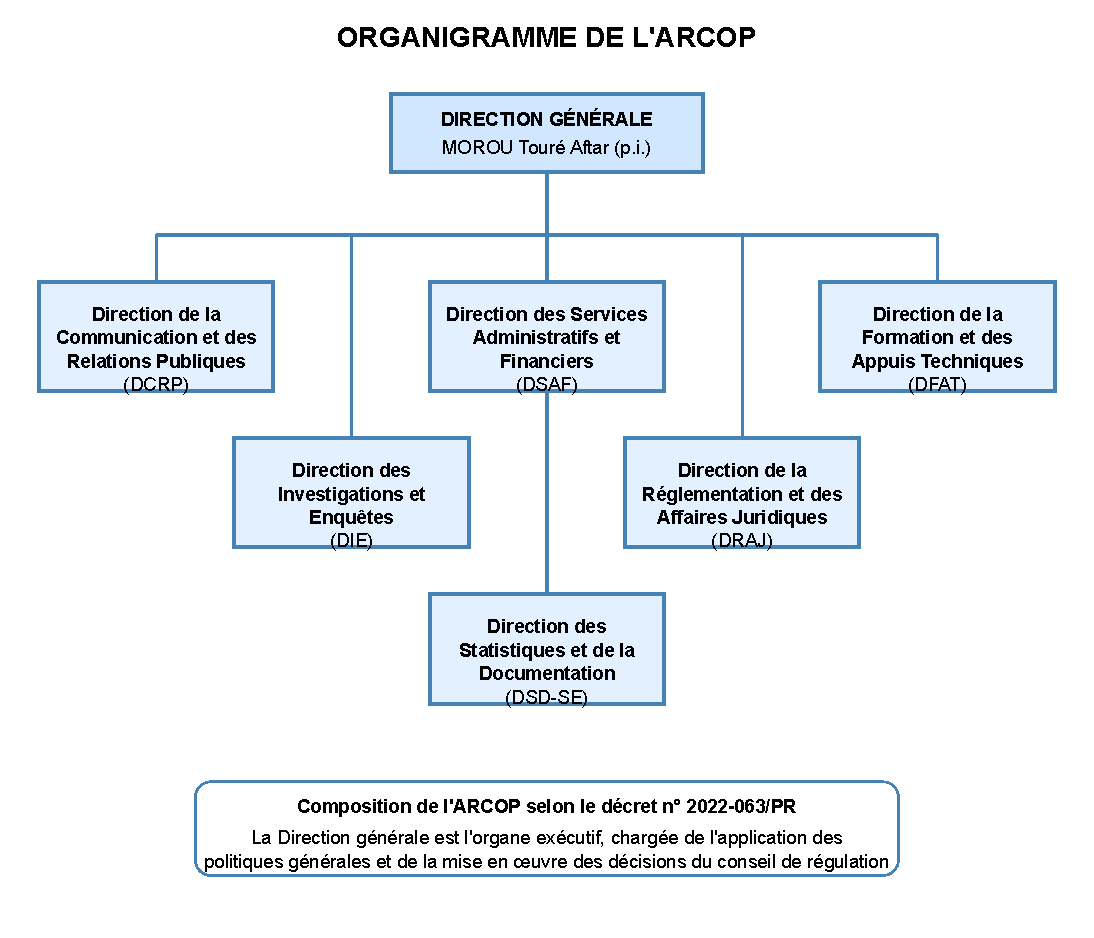
\includegraphics[width=\textwidth]{images/diagrammes/autres/organigramme-arcop.pdf}
    \caption{Organigramme de la Direction générale de l'\ac{ARCOP}}
    \label{fig:organigramme-arcop}
\end{figure}

La Direction générale de l’\ac{ARCOP} exerce une surveillance active sur les processus d'achat public afin de garantir l'intégrité, la transparence et l'efficacité des dépenses publiques, contribuant ainsi au développement économique et social du pays.



\clearpage
%-------------------------------------------------------------------+
\chapter{Déroulement factuel du stage}
\clearpage


\section{Prise de fonction et intégration}
À l'arrivée au sein de l'\ac{ARCOP}, l'intégration s'est effectuée au sein de la Direction des Statistiques et de la Documentation. Une présentation de l'organisation et des missions du service a permis de mieux comprendre son fonctionnement. Les objectifs du stage ainsi que les attentes du tuteur ont ensuite été exposés.
Durant cette phase d'intégration, plusieurs actions ont été réalisées :

\begin{itemize}
    \item Découvert l'environnement de travail et les outils utilisés.
    \item Pris en main les méthodologies internes et les processus en place.
    \item Échangé avec les membres de l'équipe pour mieux comprendre les besoins et le cadre du stage.

\end{itemize}
\section{Tâches effectuées}
Tout au long du stage à la Direction des Statistiques et de la Documentation de l'\ac{ARCOP}, plusieurs tâches ont été effectuées, notamment:
\begin{itemize}
    \item Installation et maintenance des équipements informatiques
    \item Développement Web
    \item Débogage du réseau téléphonique IP de l'entreprise 
    \item Support aux utilisateurs de la \ac{PASSE}
    \item Assistance technique générale    
\end{itemize} 
\subsection{Installation et maintenance des équipements informatiques}
Cette mission a consisté à assurer le bon fonctionnement du matériel informatique en effectuant :
\begin{itemize}
    \item L’installation et la configuration des ordinateurs de bureau pour les employés.

    \item La mise en place et la mise à jour des logiciels antivirus afin de garantir la sécurité des données.
    \item Le diagnostic et la résolution des pannes matérielles et logicielles.
\end{itemize}
\subsection{Développement Web}
\subsubsection{Découverte du projet principal et études préliminaires}
L'objectif principal de mon stage était la \textbf{digitalisation des processus de travail du département des \ac{RH}}. Avant d'entamer le développement, plusieurs tâches préparatoires ont été réalisées :




\begin{itemize}
    \item Analyse des besoins du département en collaboration avec le responsable du département des \ac{RH}.
    \item Étude des solutions existantes et identification des axes d'amélioration.
    \item Participation aux réunions pour recueillir les attentes des utilisateurs.
    \item Rédaction d'un cahier des charges et validation des fonctionnalités essentielles avec mon tuteur.
\end{itemize}

\subsubsection{Développement de la solution numérique}
Après cette phase d'étude, j'ai entamé la conception et le développement de l'application. Cela a inclus :
\begin{itemize}
    \item La mise en place de l'environnement de développement (choix des technologies, configuration des outils).
    \item La conception de l'architecture du projet et de la base de données.
    \item Le développement des premières fonctionnalités, notamment \textbf{ l'authentification et la gestion des utilisateurs}.
    \item Des tests et des ajustements basés sur les retours du tuteur et des futurs utilisateurs.

\end{itemize}
Par la suite, d'autres fonctionnalités ont été intégrées, comme :

\begin{itemize}
    \item La gestion des documents administratifs.
    \item L'automatisation de certaines tâches du département des \ac{RH}.
    \item L'amélioration de l'interface utilisateur pour une meilleure expérience.
\end{itemize}
\subsubsection{Finalisation du projet et restitution}
Dans les dernières semaines du stage, mon travail s'est concentré sur :

\begin{itemize}
    \item La finalisation du développement et la correction des derniers bugs.
    \item La rédaction de la documentation technique et utilisateur.
    \item La présentation du projet aux responsables du département des \ac{RH} et la collecte des feedbacks.
    \item La formation des collaborateurs à l'utilisation de la solution développée.

\end{itemize}
\subsection{Débogage du réseau téléphonique IP de l'entreprise}
Afin d’assurer le bon fonctionnement des communications internes, une intervention sur le réseau téléphonique IP a été menée :
\begin{itemize}
    \item Analyse des dysfonctionnements et identification des causes des interruptions de service.
    \item  Participation aux interventions techniques visant à rétablir la connexion et  la qualité des appels.
    \item Assistance aux utilisateurs pour résoudre les problèmes liés à la téléphonie IP
\end{itemize}


\subsection{Support aux utilisateurs de la \acs{PASSE}}

\subsubsection{Présentation de la PASSE}
La \textbf{\ac{PASSE}} (\textit{Plateforme de l’ARCOP pour des Services Sécurisés et Électroniques}) est un outil numérique conçu pour optimiser la gestion et le suivi des services économiques. Elle permet aux opérateurs économiques d’effectuer diverses démarches administratives en ligne et d’accéder aux informations essentielles liées à leurs activités, notamment la demande d’attestation de régularité de la taxe parafiscale.

La plateforme est accessible via le lien suivant :  
\url{https://passe.arcop.tg}  

\subsubsection{Accompagnement des utilisateurs}
Afin d’assurer une utilisation optimale de la plateforme et garantir une expérience fluide aux opérateurs économiques, un dispositif de support et d’assistance technique a été mis en place :

\begin{itemize}
    \item \textbf{Participation au comité de suivi de la \ac{PASSE}} : Contribution active aux échanges et décisions visant à améliorer le fonctionnement et l'efficacité de la plateforme.
    
    \item \textbf{Assistance technique} : Un accompagnement personnalisé est proposé aux opérateurs économiques, notamment pour l’accès à la plateforme, la soumission des documents et l’utilisation des différents services en ligne.
\end{itemize}


\subsubsection{Captures d'écran}
Pour mieux illustrer l'interface et les principales fonctionnalités de la \ac{PASSE}, voici quelques captures d’écran :

\begin{figure}[H]
    \centering
    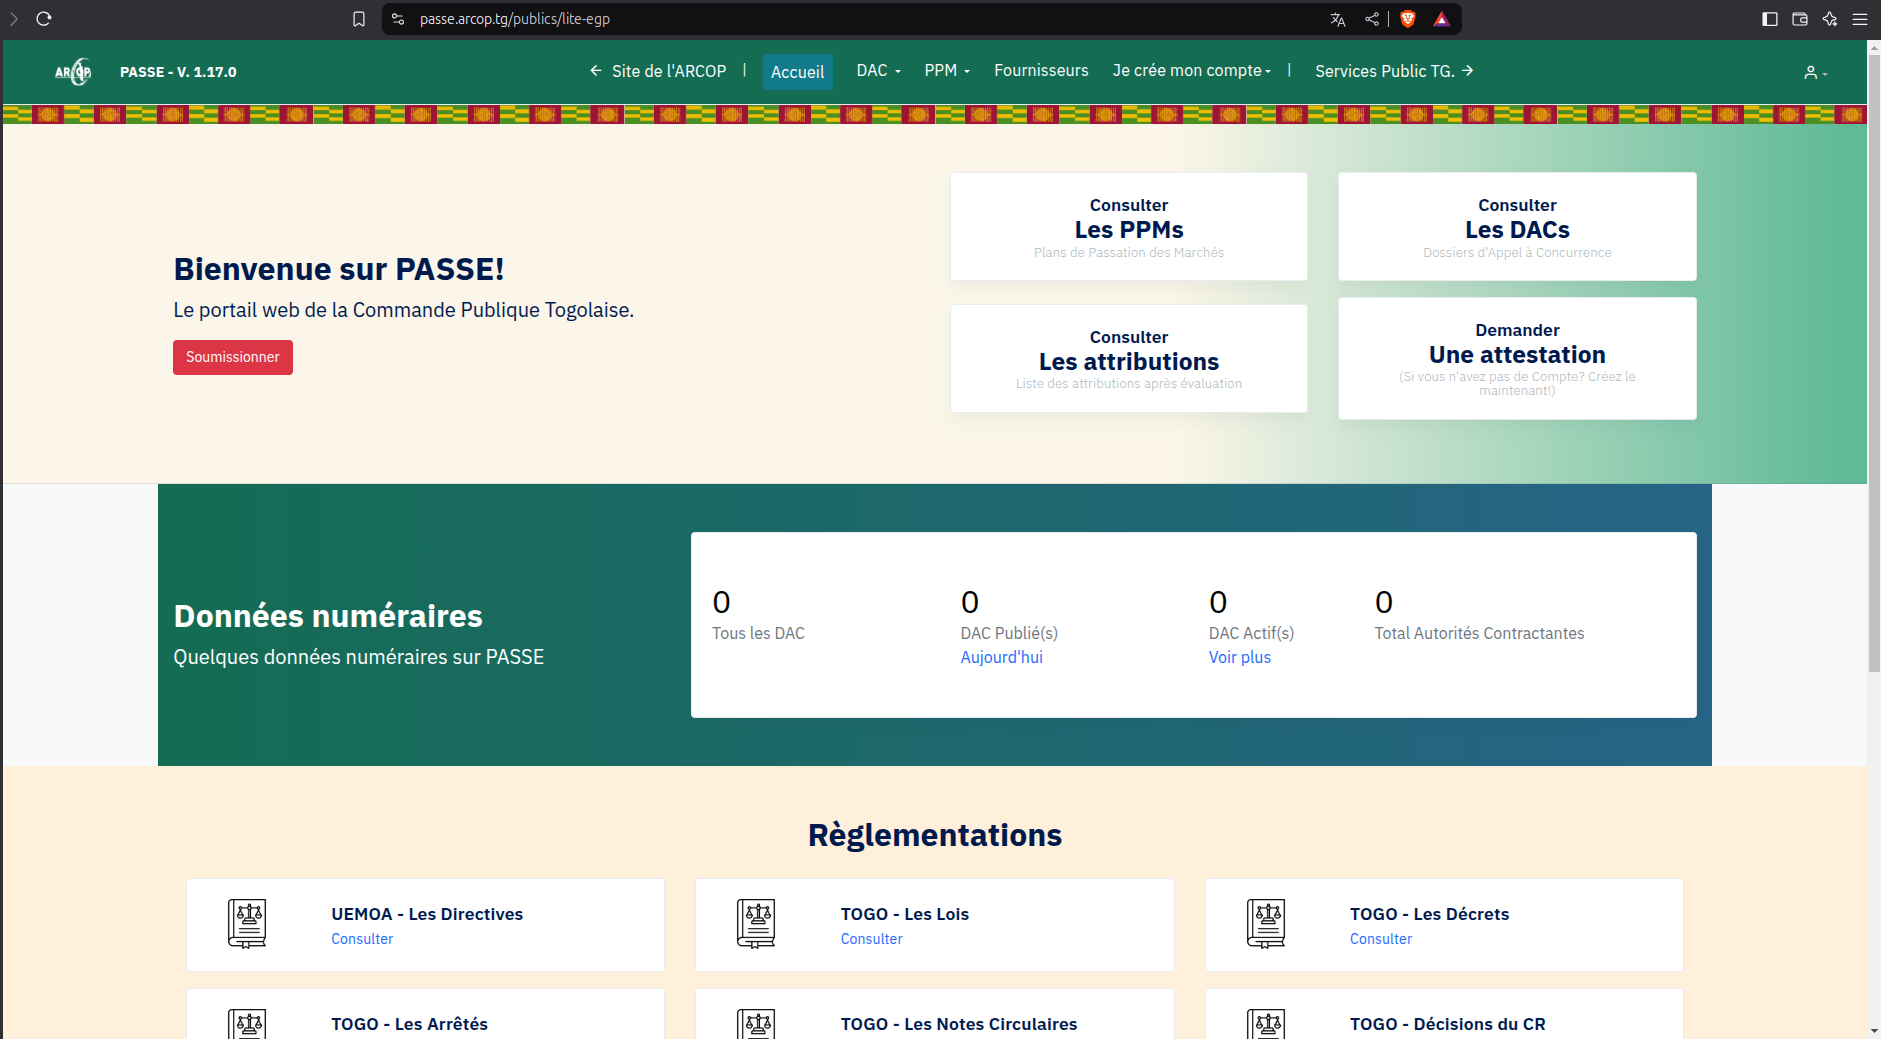
\includegraphics[width=0.8\textwidth]{images/passe/home.png}
    \caption{Page d'accueil de la \ac{PASSE}}
    \label{fig:page-accueil_pass}
\end{figure}

\begin{figure}[H]
    \centering
    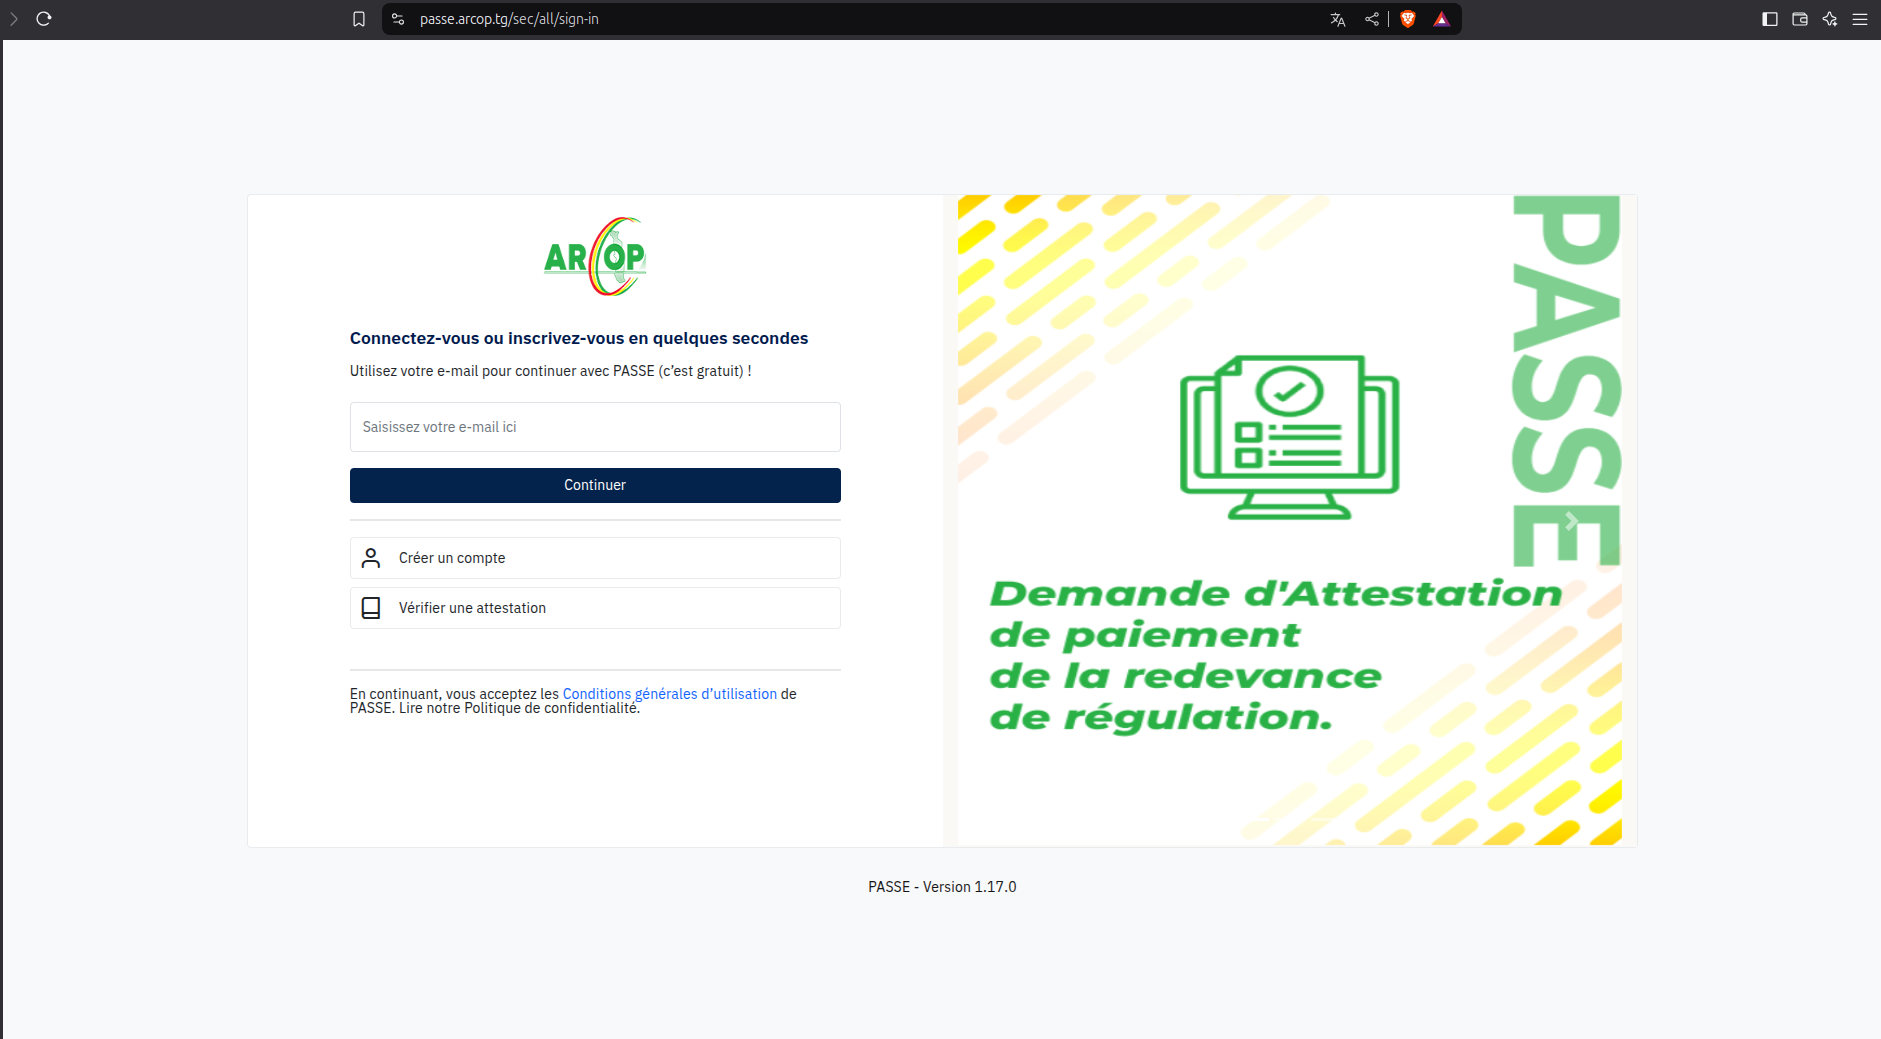
\includegraphics[width=0.8\textwidth]{images/passe/login.png}
    \caption{Interface de connexion de la \ac{PASSE}}
    \label{fig:interface-login_pass}
\end{figure}








\subsection{Assistance technique générale}
En complément des missions spécifiques, un support technique global a été assuré au sein de l’organisation :
\begin{itemize}
    \item Dépannage et maintenance des outils informatiques utilisés par le personnel.
    \item Configuration et optimisation des postes de travail selon les besoins des employés.
    \item Sensibilisation aux bonnes pratiques pour garantir la pérennité des équipements et la sécurité des données.
\end{itemize}
\section{Remarques et suggestions}

Au terme de ce stage au sein de la Direction des Statistiques et de la Documentation de l'ARCOP, plusieurs observations et recommandations peuvent être formulées dans une perspective d'amélioration continue.

\subsection{Concernant l'infrastructure informatique}

\begin{itemize}
    \item \textbf{Renouvellement planifié du parc informatique} : Certains équipements atteignent leur limite d'âge et nécessiteraient un plan de renouvellement progressif pour éviter les interruptions de service.
    
    \item \textbf{Consolidation de la sécurité informatique} : La mise en place d'une politique de sécurité plus robuste, incluant des formations régulières pour les utilisateurs, permettrait de réduire les risques liés aux cybermenaces.
    
    \item \textbf{Optimisation du réseau téléphonique IP} : Suite aux interventions effectuées, il serait judicieux d'investir dans une solution plus stable et moderne pour garantir la fiabilité des communications internes.
\end{itemize}



\subsection{À propos de la Plateforme PASSE}

\begin{itemize}
    \item \textbf{Amélioration de l'expérience utilisateur} : L'interface de la PASSE gagnerait à être simplifiée pour les opérateurs économiques moins familiers avec les outils numériques.
    
    \item \textbf{Documentation utilisateur enrichie} : La création de guides détaillés et de tutoriels vidéo permettrait de réduire le nombre de sollicitations auprès du support technique.
    
    \item \textbf{Mise en place d'un système de feedback} : L'intégration d'un mécanisme permettant aux utilisateurs de signaler les problèmes ou suggérer des améliorations contribuerait à l'évolution positive de la plateforme.
\end{itemize}

\subsection{Remarques générales}

\begin{itemize}
    \item \textbf{Standardisation des procédures} : L'élaboration de procédures standardisées pour la gestion des incidents informatiques optimiserait le temps de résolution et garantirait une qualité de service constante.
    
    \item \textbf{Veille technologique} : La mise en place d'une veille active sur les innovations technologiques pertinentes pour l'ARCOP permettrait d'anticiper les évolutions nécessaires.
\end{itemize}

Ces suggestions s'inscrivent dans une démarche d'amélioration continue visant à optimiser l'efficacité des processus et la qualité des services proposés par l'ARCOP, tant en interne qu'auprès des opérateurs économiques.




\section{Bilan et conclusion}
Cette expérience a permis de mieux appréhender les enjeux liés à la gestion d’un service informatique, alliant assistance aux utilisateurs, maintenance technique et développement d’outils numériques.

\clearpage

%-------------------------------------------------------------------+
\chapter{Expression des besoins}
\clearpage
\section{introduction}

L'objectif de ce projet est de développer un logiciel de gestion des \ac{RH} pour l'(\ac{ARCOP}). Ce logiciel permettra de centraliser et d'automatiser la gestion des congés, des absences, des formations, et des évaluations des employés, en s'adressant directement aux employés et au département de la Gestion des Ressources Humaines (GRH).
\section{Spécifications}
\subsection{Spécifications Fonctionnelles}


\subsubsection{Gestion des Congés et Absences}
\begin{itemize}
    \item \textbf{Mise à jour du planning et du solde des congés :} Le logiciel doit permettre aux employés de l'\ac{ARCOP} de demander des congés en ligne, avec une mise à jour du planning et du solde de congés. Les demandes seront soumises au supérieur, puis au DG après approbation du GRH.

    
    \item \textbf{Rapports personnalisables :} Le logiciel offrira la possibilité de générer des rapports sur la durée, la fréquence, et les motifs des congés, personnalisables selon les besoins du GRH.
    

    
  
\end{itemize}

\subsubsection{Gestion des dossiers}
\begin{itemize}
    \item \textbf{Dossier personnalisé en ligne pour chaque agent :} Un dossier en ligne pour chaque employé de l'\ac{ARCOP} sera accessible via la version web du logiciel, contenant toutes les informations concernant ses congés, absences, et autres données des \ac{RH}.
    
    \item \textbf{Téléchargement des bulletins de paie :} Extraction des bulletins de paie depuis Sage Paie, puis les rendre disponibles aux employés dans l'application après un chargement.
    \item \textbf{Demande de documents administratifs :} Les employés
    pourront demander des documents administratifs en ligne, tels que des attestations de travail, des certificats de travail.
\end{itemize}

\subsubsection{Publication des notes et informations}
\begin{itemize}
    \item \textbf{Publication des notes et informations :} Le GRH pourra publier des notes, des informations, et des documents des \ac{RH} pour les employés, accessibles via l'interface web du logiciel.
    \item \textbf{Alertes et notifications :} Les employés recevront des alertes et des notifications pour les rappeler des échéances, des actions sur les demandes.
\end{itemize}

\subsection{Spécifications techniques}

\subsubsection{Langages et Technologies}
\begin{itemize}
    \item \textbf{Framework :} Laravel pour une gestion efficace de la logique serveur et du backend.
    \item \textbf{Base de données :} MySQL ou PostgreSQL pour la gestion des données avec Eloquent ORM.
    \item \textbf{Frontend :} Blade pour une interface utilisateur dynamique et fluide.

\end{itemize}


\subsubsection{Sécurité}
\begin{itemize}
    \item Chiffrement des données sensibles.
    \item Gestion des accès par rôles.
\end{itemize}

\subsubsection{Hébergement}
\begin{itemize}
    \item Déploiement sur les serveurs internes de l'\ac{ARCOP}.
\end{itemize}
\subsection{Exigences non fonctionnelles}


\subsubsection{Fiabilité}
\begin{itemize}
    \item Le logiciel doit être disponible 99.9\% du temps, excluant les périodes de maintenance planifiée.
    \item Les données doivent être sauvegardées quotidiennement avec une possibilité de restauration en cas de panne.
\end{itemize}

\subsubsection{Utilisabilité}
\begin{itemize}
    \item L'interface utilisateur doit être intuitive et facile à utiliser, avec une courbe d'apprentissage minimale.
    \item Une documentation utilisateur complète doit être fournie, incluant des guides et des tutoriels.
\end{itemize}

\subsubsection{Compatibilité}
\begin{itemize}
    \item \textbf{Navigateurs :} Le logiciel doit être compatible avec les dernières versions de Chrome, Firefox, Safari, et Edge.
    \item \textbf{Mobile :} L'application web doit être responsive et accessible depuis les navigateurs mobiles.
\end{itemize}

\subsubsection{Scalabilité}
Le logiciel doit pouvoir gérer un nombre croissant d'utilisateurs et de données sans dégradation des performances.


\subsubsection{Nom du logicièl}
Le logiciel sera nommé \textbf{OptiHR}, un nom qui allie modernité et professionnalisme, reflétant une gestion
optimale des ressources humaines.


\section{Définition des acteurs systèmes}
Le logiciel est destiné aux employés de l’\ac{ARCOP} et au département de la Gestion des Ressources Humaines (GRH), facilitant une gestion efficace des congés, de la formation, et des évaluations.
Les utilisateurs principaux du systemes sont:
\begin{itemize}
    \item Employé 
    \item GRH 
    \item DSAF 
    \item DG 
\end{itemize}
\subsection{Employé}
L'utilisateur \textbf{Employé} désignent un employé de l'\ac{ARCOP}. Il utilisent le logiciel pour demander des congés, demander des documents, suivre des formations, et participer aux évaluations. Ils accèdent à leur dossier personnel en ligne pour consulter leur solde de congés, leurs absences, et leurs évaluations.
\subsection{GRH}
Le \textbf{GRH} désigne le \textbf{Chef division des ressources humaines et services généraux} de l'\ac{ARCOP}. Il utilise le logiciel pour gérer les demandes de congés,les documents, les formations, et les évaluations des employés. Il peut consulter les rapports des \ac{RH}, planifier les entretiens,publier des notes ou informations, et suivre les indicateurs de performance.
\subsection{DSAF }
Le \textbf{DSAF} désigne le \textbf{ Directeur des services administratif et financier} de l'\ac{ARCOP}. Il utilise le logiciel pour suivre les demandes effectuées par les employées. IL interagite principallement en consultation.
\subsection{DG}
Le \textbf{DG} désigne le \textbf{Directeur Général} de l'\ac{ARCOP}. Il utilise le logiciel pour valider les demandes de congés, les budgets de formation, et les résultats des évaluations. Il peut consulter les rapports des \ac{RH} et financiers pour prendre des décisions stratégiques en matière de ressources humaines.


\section{D\'efinition des cas d'utilisation}

Un diagramme de cas d'utilisation est une représentation graphique des interactions entre les acteurs d'un système et ses fonctionnalités. Il permet d'identifier et de structurer les besoins fonctionnels du logiciel en décrivant les actions réalisées par chaque acteur. Ce type de diagramme est particulièrement utile pour comprendre les interactions des utilisateurs avec le système et pour définir clairement les responsabilités de chaque acteur.

Dans ce contexte, nous définissons les cas d'utilisation pour chaque fonctionnalités énoncés précédemment.
\subsection{Gestion des Congés et Absences}
\subsubsection{Description de la fonctionnalité}
La gestion des congés et des absences est une fonctionnalité essentielle du logiciel, permettant aux employés de demander des congés en ligne, de consulter leur solde de congés, et de générer des rapports sur les congés et les absences.
\subsubsection{Description des cas d'utilisation}
\begin{itemize}
    \item \textbf{Demande de congé :} L'employé peut demander un congé en ligne, en précisant la date, la durée, et le motif.
    \item \textbf{Annulation de la demande de congé :} L'employé peut annuler sa demande de congé en ligne tant que son supérieur hiérarchique n'a pas encore effectué d'action.
    \item \textbf{approbation du supérieur :} Le supérieur hiérarchique peut valider ou refuser la demande de congé de l'employé.
    \item \textbf{Approbation du GRH :} Le GRH peut valider ou refuser la demande de congé après approbation du supérieur.
    \item \textbf{Validation du DG :} Le DG peut valider ou refuser la demande de congé après approbation du GRH.
    \item \textbf{Consultation du solde de congés :} L'employé peut consulter son solde de congés et les congés déjà pris.
    \item \textbf{Génération de rapports :} Le GRH peut générer des rapports sur les congés, les absences, et les motifs.
    \item \textbf{Télécharger le document de validation :} L'employé peut télécharger le pdf de validation de la demande de congés ou absences.
\end{itemize}
\subsubsection{Diagramme de cas d'utilisation}
\begin{figure}[H]
    \centering
    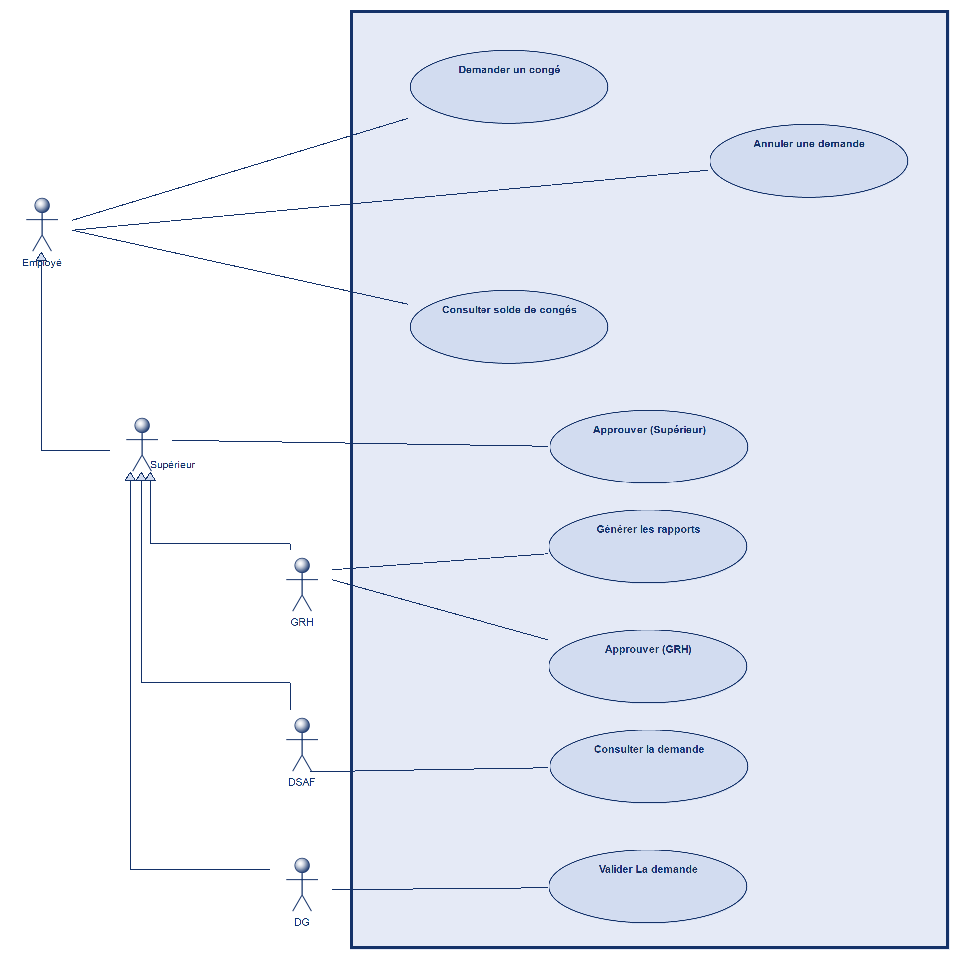
\includegraphics[width=0.8\textwidth]{images/diagrammes/use-cases/conges.png}
    \caption{Diagramme de cas d'utilisation Gestion des Congés et Absences}
    \label{fig:use_case_gestion_conges}

\end{figure}
\subsubsection{Diagramme de processus}
Le diagramme de processus modélise les étapes d'exécution de certaines fonctionnalités clés du système. Le diagramme de processus pour la gestion des congés et des absences est le suivant :
\begin{figure}[H]
    \centering
    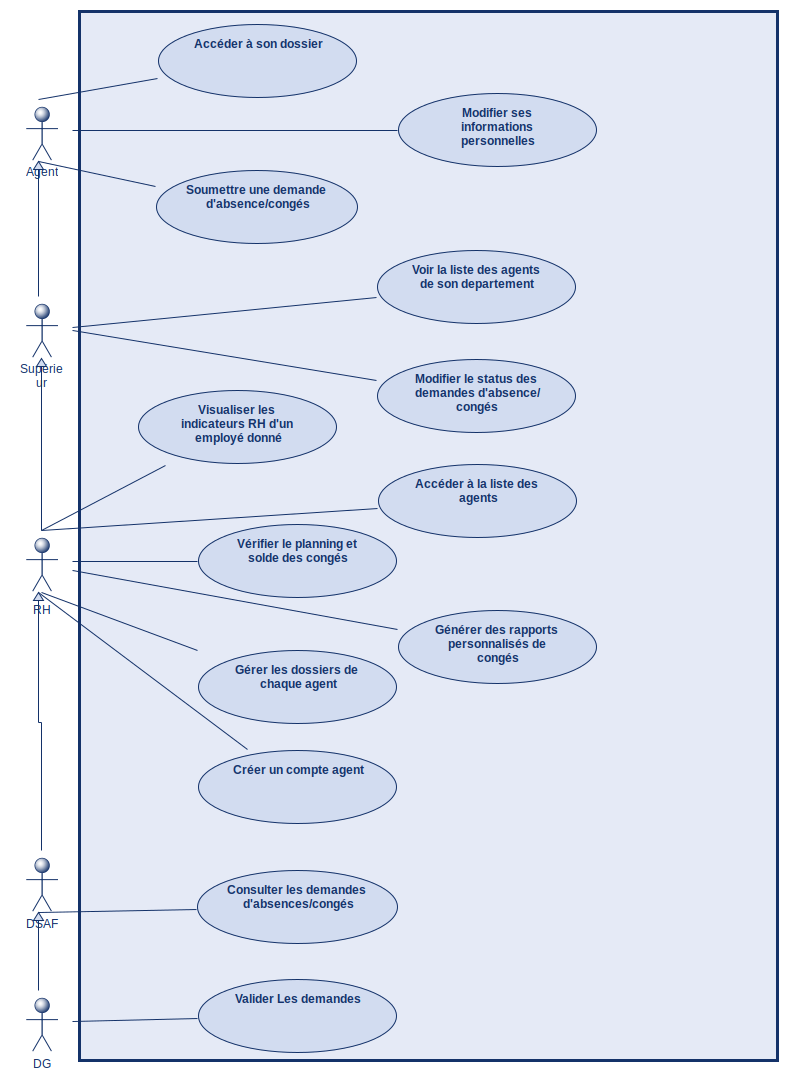
\includegraphics[width=0.8\textwidth]{images/diagrammes/flowcharts/conges.png}
    \caption{Diagramme de processus Gestion des Congés et Absences}
    \label{fig:flow_gestion_conges}
\end{figure}

\subsection{Gestion des dossiers}
\subsubsection{Description de la fonctionnalité}
La gestion des dossiers permet aux employés de consulter leur dossier personnel en ligne, de télécharger des bulletins de paie, et de demander des documents administratifs.
\subsubsection{Description des cas d'utilisation}
\begin{itemize}
    \item \textbf{Consultation du dossier personnel :} L'employé peut consulter son dossier personnel en ligne, contenant ses congés, absences, formations, et évaluations.
    \item \textbf{Téléchargement des bulletins de paie :} L'employé peut télécharger ses bulletins de paie depuis l'application.
    \item \textbf{Demande de documents administratifs :} L'employé peut demander des documents administratifs en ligne, tels que des attestations de travail, des certificats de travail.
\end{itemize}
\subsubsection{Diagramme de cas d'utilisation}
\begin{figure}[H]
    \centering
    \includegraphics[width=0.8\textwidth]{images/diagrammes/use-cases/dossiers.png}
    \caption{Diagramme de cas d'utilisation Gestion des dossiers}
    \label{fig:use_case_gestion_dossiers}
\end{figure}
\subsubsection{Diagramme de processus}
Le diagramme de processus pour la gestion des dossiers est le suivant :
\begin{figure}[H]
    \centering
    \includegraphics[width=0.8\textwidth]{images/diagrammes/flowcharts/dossiers.png}
    \caption{Diagramme de processus Gestion des dossiers}
    \label{fig:flow_gestion_dossiers}
\end{figure}
\subsection{Publication des notes et informations}
\subsubsection{Description de la fonctionnalité}
La publication des notes et des informations permet au GRH de publier des notes, des informations, et des documents des \ac{RH} pour les employés, avec des alertes et des notifications pour les rappeler des échéances.
\subsubsection{Description des cas d'utilisation}   
\begin{itemize}
    \item \textbf{Publication des notes et informations :} Le GRH peut publier des notes, des informations, et des documents des \ac{RH} pour les employés.
    \item \textbf{Alertes et notifications :} Les employés reçoivent des alertes et des notifications pour les rappeler des échéances, des actions sur les demandes.
\end{itemize}
\subsubsection{Diagramme de cas d'utilisation}
\begin{figure}[H]
    \centering
    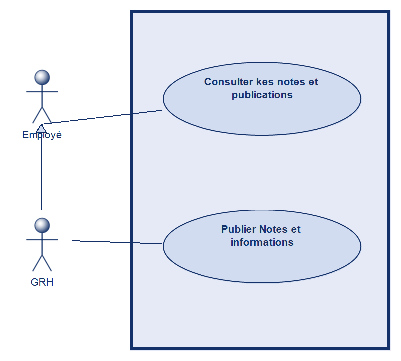
\includegraphics[width=0.8\textwidth]{images/diagrammes/use-cases/note.png}
    \caption{Diagramme de cas d'utilisation Publication des notes et informations}
    \label{fig:use_case_publication}
\end{figure}
\subsubsection{Diagramme de processus}
Le diagramme de processus pour la publication des notes et des informations est le suivant :
\begin{figure}[H]
    \centering
    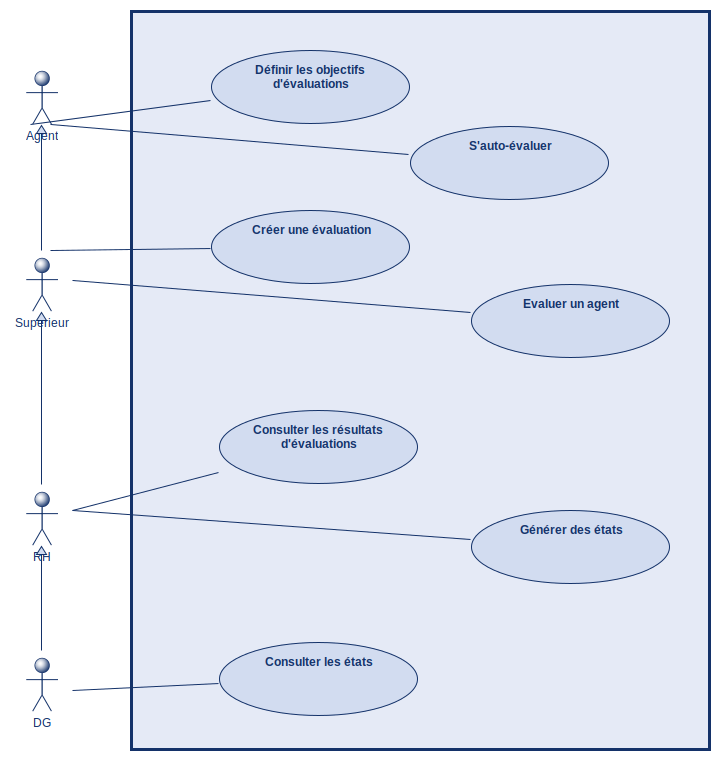
\includegraphics[width=0.8\textwidth]{images/diagrammes/flowcharts/note.png}
    \caption{Diagramme de processus Publication des notes et informations}
    \label{fig:flow_publication}
\end{figure}

\section{Conclusion}
Ce cahier des charges définit les fonctionnalités et les exigences techniques d'un logiciel de gestion des \ac{RH} performant et sécurisé pour l'\ac{ARCOP}. Le logiciel, nommé \textbf{OptiHR}, répondra aux besoins spécifiques du GRH et des employés, en facilitant la gestion des congés, des formations, et des évaluations, d'éditer les bulletins de paie tout en étant évolutif et intégrable aux systèmes existants. La prochaine étape consistera à concevoir l'architecture du système et à élaborer les diagrammes UML pour modéliser les interactions entre les différents modules.
\clearpage

%-------------------------------------------------------------------+
\chapter{Conception}
\clearpage

\section{Introduction}
La phase de conception constitue une étape déterminante dans le cycle de développement logiciel. 
Elle permet de traduire les besoins fonctionnels identifiés en une architecture technique cohérente. 
Cette étape définit non seulement l'architecture globale et les composants principaux du système, 
mais aussi les interactions entre les différents modules.

La conception du système OptiHR s'inscrit dans une démarche méthodique visant à garantir 
la qualité, la maintenabilité et l'évolutivité de la solution. Une attention particulière 
a été portée à la modélisation des données et à l'organisation des classes pour refléter 
fidèlement les processus métier de l'ARCOP.

\section{Architecture du système}

\subsection{Architecture globale}
Le système OptiHR adopte une architecture en couches qui permet une séparation claire des responsabilités:

\begin{itemize}
    \item \textbf{Couche Présentation}: Interfaces utilisateur accessibles via navigateur web, incluant les templates Blade, les feuilles de style CSS et le code JavaScript.
    \item \textbf{Couche Application}: Logique métier et traitement des requêtes via les contrôleurs Laravel et les services métier.
    \item \textbf{Couche Persistance}: Stockage et récupération des données à travers l'ORM Eloquent et la base de données PostgreSQL.
\end{itemize}

Cette architecture en trois couches favorise la modularité et facilite la maintenance du code en isolant 
les changements à des zones spécifiques du système.

\begin{figure}[H]
    \centering
    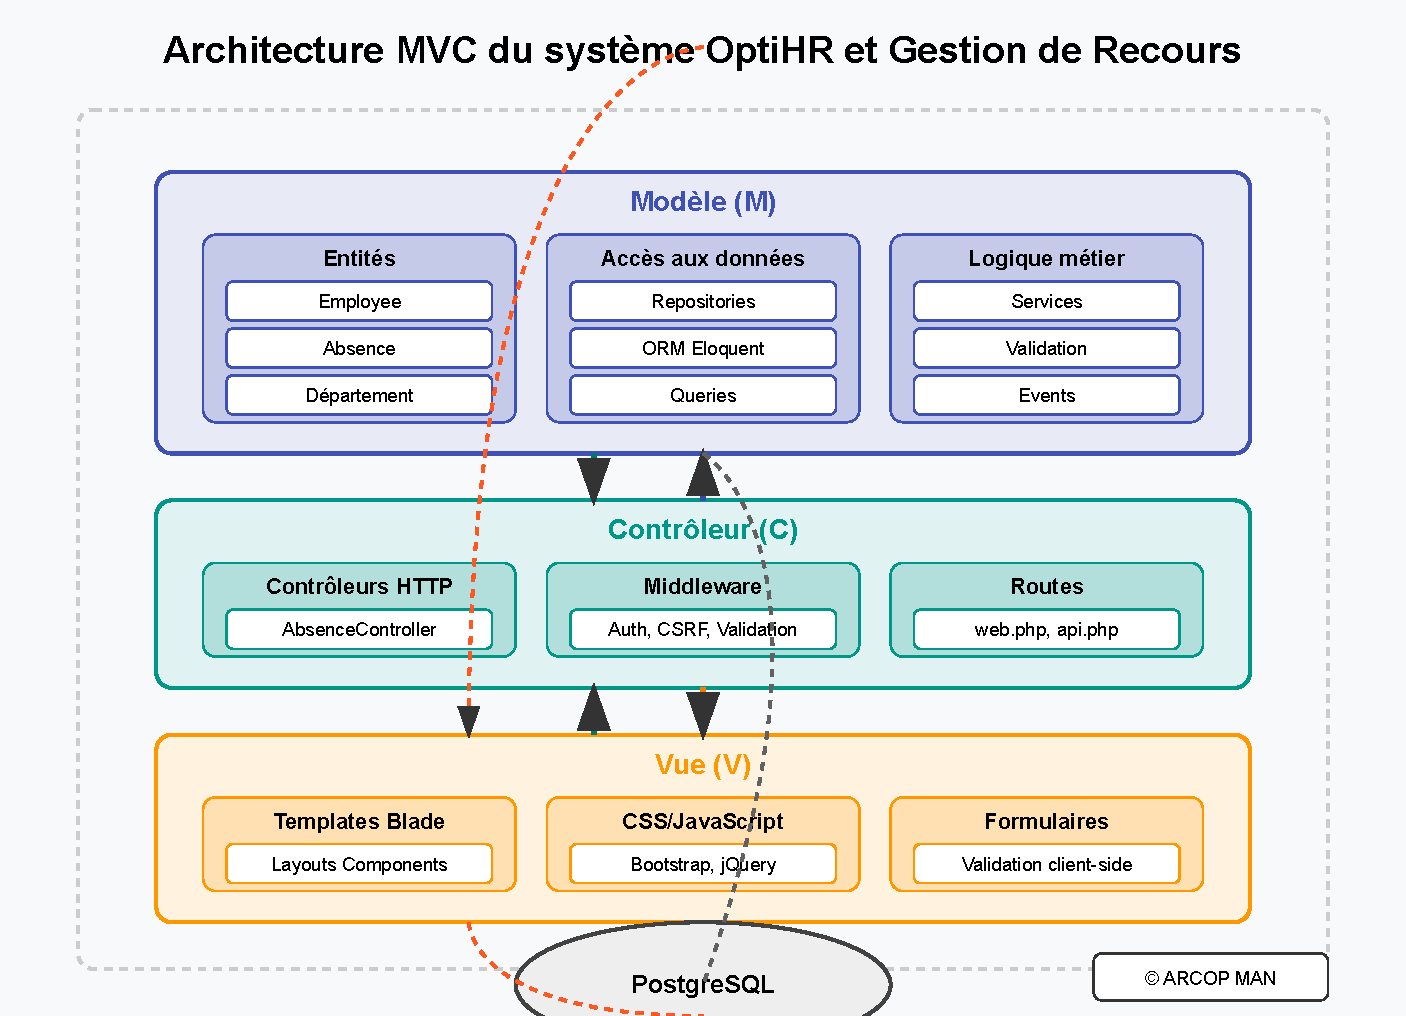
\includegraphics[width=0.9\textwidth]{images/diagrammes/architecture/architecture-couches.pdf}
    \caption{Architecture en couches du système OptiHR}
    \label{fig:architecture_couches}
\end{figure}

La figure \ref{fig:architecture_couches} illustre comment les différentes couches interagissent entre elles, avec un flux de données descendant pour les requêtes et ascendant pour les réponses. Les flèches représentent les dépendances entre les composants.

\subsection{Découpage modulaire du système}
Pour favoriser la maintenabilité et l'évolutivité, le système OptiHR est conçu selon une approche 
modulaire qui sépare les différentes préoccupations fonctionnelles:

\begin{enumerate}
    \item \textbf{Module d'authentification et autorisations}: Gestion des utilisateurs, des rôles et des permissions.
    \item \textbf{Module GRH}: Gestion des employés, des départements et de la documentation.
    \item \textbf{Module de gestion des absences}: Demandes de congés, workflow d'approbation et suivi.
    \item \textbf{Module de notifications}: Alertes système, notifications par email et notes de service.
    \item \textbf{Module documentaire}: Bulletins de paie, documents administratifs et archivage.
\end{enumerate}

\begin{figure}[H]
    \centering
    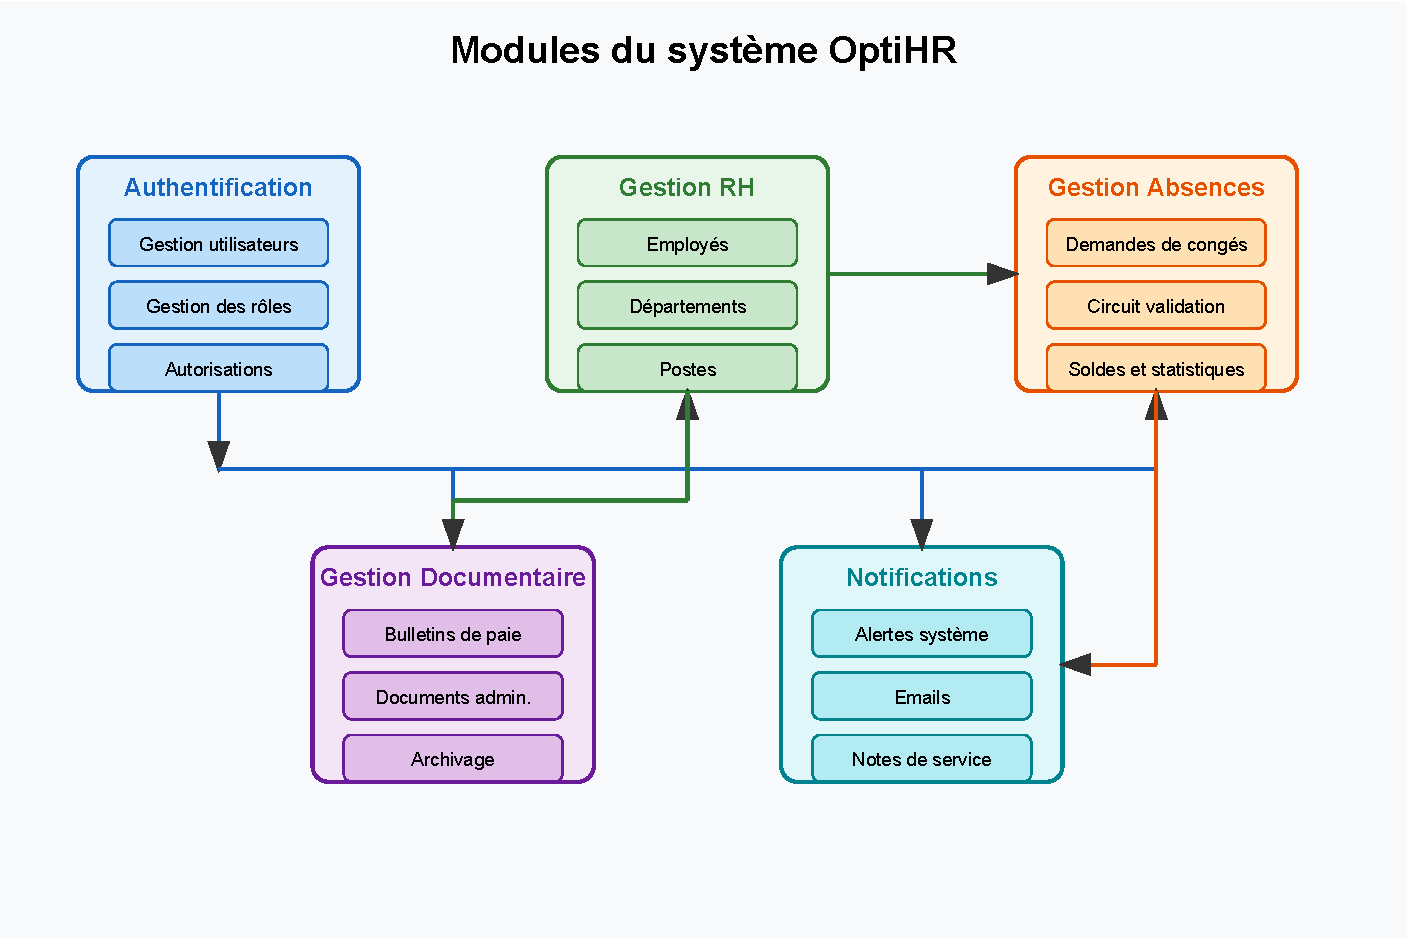
\includegraphics[width=0.9\textwidth]{images/diagrammes/architecture/modules-systeme.pdf}
    \caption{Organisation modulaire du système OptiHR}
    \label{fig:modules_systeme}
\end{figure}

Cette organisation modulaire, illustrée dans la figure \ref{fig:modules_systeme}, permet d'isoler les fonctionnalités 
et de faciliter les évolutions futures du système en minimisant les impacts entre modules.

\subsection{Flux de données et interactions}
Les interactions entre les composants suivent un flux standardisé qui garantit la cohérence des opérations
et facilite le débogage:

\begin{figure}[H]
    \centering
    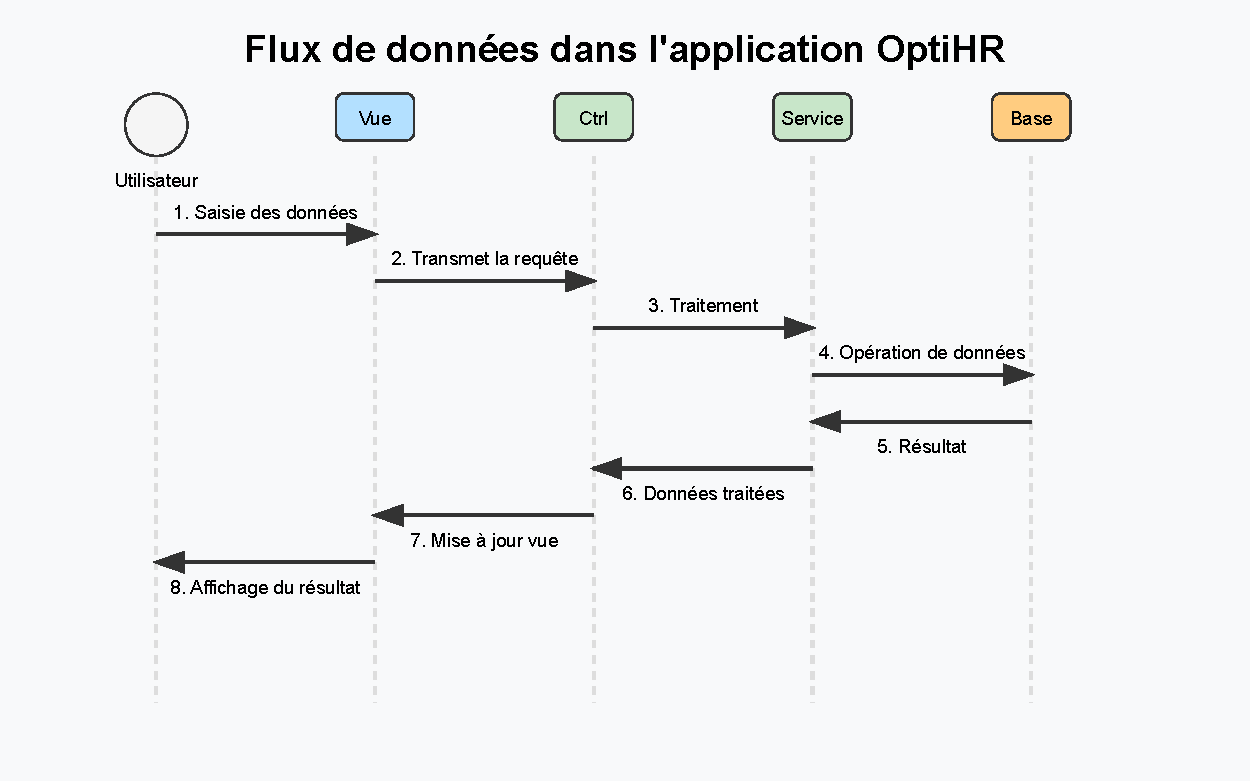
\includegraphics[width=0.9\textwidth]{images/diagrammes/architecture/flux-donnees.pdf}
    \caption{Flux de données dans l'application OptiHR}
    \label{fig:flux_donnees}
\end{figure}

Le diagramme de séquence (figure \ref{fig:flux_donnees}) détaille le parcours d'une requête typique à travers les différentes couches du système:

\begin{enumerate}
    \item L'utilisateur interagit avec l'interface (Vue)
    \item Les requêtes sont acheminées vers le Contrôleur approprié
    \item Le Contrôleur délègue le traitement aux Services
    \item Les Services manipulent les données via le Modèle
    \item Le Modèle interagit avec la base de données
    \item Les données sont remontées à travers les couches
    \item L'interface est mise à jour avec les résultats
    \item Le résultat final est affiché à l'utilisateur
\end{enumerate}


\section{Modélisation des données}

\subsection{Dictionnaire de données}
Le dictionnaire de données ci-dessous détaille les structures de stockage avec leurs attributs, 
types, contraintes et descriptions. Cette documentation précise garantit l'intégrité et 
la cohérence des données manipulées par le système.

\renewcommand{\arraystretch}{1.3} % Améliore l'espacement du tableau

\begin{longtable}{|p{2.5cm}|p{3cm}|p{3cm}|p{3cm}|p{3cm}|}
    \hline
    \textbf{Table} & \textbf{Attribut} & \textbf{Type SQL} & \textbf{Contrainte} & \textbf{Description} \\
    \hline
    \endfirsthead

    \hline
    \textbf{Table} & \textbf{Attribut} & \textbf{Type SQL} & \textbf{Contrainte} & \textbf{Description} \\
    \hline
    \endhead

    % User
    \multirow{5}{*}{\textbf{User}} & id & INT & PK, AUTO\_INCREMENT & Identifiant unique \\
    \cline{2-5}
    & username & VARCHAR(50) & NOT NULL, UNIQUE & Nom d'utilisateur \\
    \cline{2-5}
    & password & VARCHAR(255) & NOT NULL & Mot de passe haché \\
    \cline{2-5}
    & active & BOOLEAN & NOT NULL, DEFAULT TRUE & Statut du compte \\
    \cline{2-5}
    & employee\_id & INT & FK(Employee.id) & Référence à l'employé \\
    \hline

    % Employee
    \multirow{12}{*}{\textbf{Employee}} & id & INT & PK, AUTO\_INCREMENT & Identifiant unique \\
    \cline{2-5}
    & first\_name & VARCHAR(50) & NOT NULL & Prénom \\
    \cline{2-5}
    & last\_name & VARCHAR(50) & NOT NULL & Nom de famille \\
    \cline{2-5}
    & phone\_number & VARCHAR(20) & NULL & Numéro de téléphone \\
    \cline{2-5}
    & email & VARCHAR(100) & NOT NULL, UNIQUE & Adresse email \\
    \cline{2-5}
    & address1 & VARCHAR(255) & NULL & Adresse principale \\
    \cline{2-5}
    & address2 & VARCHAR(255) & NULL & Adresse secondaire \\
    \cline{2-5}
    & city & VARCHAR(50) & NULL & Ville \\
    \cline{2-5}
    & country & VARCHAR(50) & NULL & Pays \\
    \cline{2-5}
    & state & VARCHAR(50) & NULL & Région ou état \\
    \cline{2-5}
    & bank\_name & VARCHAR(100) & NULL & Nom de la banque \\
    \cline{2-5}
    & rib & VARCHAR(50) & NULL & RIB \\
    \cline{2-5}
    & department\_id & INT & FK(Department.id) & Département \\
    \hline

    % Department
    \multirow{3}{*}{\textbf{Department}} & id & INT & PK, AUTO\_INCREMENT & Identifiant unique \\
    \cline{2-5}
    & name & VARCHAR(100) & NOT NULL, UNIQUE & Nom du département \\
    \cline{2-5}
    & director\_id & INT & FK(Employee.id), NULL & Directeur \\
    \hline

    % Role
    \multirow{2}{*}{\textbf{Role}} & id & INT & PK, AUTO\_INCREMENT & Identifiant unique \\
    \cline{2-5}
    & name & VARCHAR(50) & NOT NULL, UNIQUE & Nom du rôle \\
    \hline

    % Permission
    \multirow{2}{*}{\textbf{Permission}} & id & INT & PK, AUTO\_INCREMENT & Identifiant unique \\
    \cline{2-5}
    & name & VARCHAR(50) & NOT NULL, UNIQUE & Nom de la permission \\
    \hline

    % Role_Permission
    \multirow{2}{*}{\textbf{Role\_Permission}} & role\_id & INT & PK, FK(Role.id) & Référence au rôle \\
    \cline{2-5}
    & permission\_id & INT & PK, FK(Permission.id) & Référence à la permission \\
    \hline

    % User_Role
    \multirow{2}{*}{\textbf{User\_Role}} & user\_id & INT & PK, FK(User.id) & Référence à l'utilisateur \\
    \cline{2-5}
    & role\_id & INT & PK, FK(Role.id) & Référence au rôle \\
    \hline

    % File
    \multirow{6}{*}{\textbf{File}} & id & INT & PK, AUTO\_INCREMENT & Identifiant unique \\
    \cline{2-5}
    & name & VARCHAR(255) & NOT NULL & Nom du fichier \\
    \cline{2-5}
    & url & VARCHAR(255) & NOT NULL & URL du fichier \\
    \cline{2-5}
    & mime\_type & VARCHAR(100) & NOT NULL & Type MIME \\
    \cline{2-5}
    & path & VARCHAR(255) & NOT NULL & Chemin d'accès \\
    \cline{2-5}
    & upload\_date & DATETIME & NOT NULL & Date d'upload \\
    \cline{2-5}
    & employee\_id & INT & FK(Employee.id) & Propriétaire \\
    \hline

    % Duty
    \multirow{5}{*}{\textbf{Duty}} & id & INT & PK, AUTO\_INCREMENT & Identifiant unique \\
    \cline{2-5}
    & duration & VARCHAR(50) & NOT NULL & Durée de la mission \\
    \cline{2-5}
    & begin\_date & DATE & NOT NULL & Date de début \\
    \cline{2-5}
    & type & VARCHAR(50) & NOT NULL & Type de mission \\
    \cline{2-5}
    & etat & VARCHAR(50) & NOT NULL & État de la mission \\
    \cline{2-5}
    & employee\_id & INT & FK(Employee.id) & Employé concerné \\
    \hline

    % Job
    \multirow{3}{*}{\textbf{Job}} & id & INT & PK, AUTO\_INCREMENT & Identifiant unique \\
    \cline{2-5}
    & title & VARCHAR(100) & NOT NULL & Intitulé du poste \\
    \cline{2-5}
    & supervisor\_id & INT & FK(Job.id), NULL & Poste supérieur \\
    \hline

    % Employee_Job
    \multirow{2}{*}{\textbf{Employee\_Job}} & employee\_id & INT & PK, FK(Employee.id) & Référence à l'employé \\
    \cline{2-5}
    & job\_id & INT & PK, FK(Job.id) & Référence au poste \\
    \hline

    % Absence
    \multirow{12}{*}{\textbf{Absence}} & id & INT & PK, AUTO\_INCREMENT & Identifiant unique \\
    \cline{2-5}
    & day\_requested & INT & NOT NULL & Jours demandés \\
    \cline{2-5}
    & start\_date & DATE & NOT NULL & Date de début \\
    \cline{2-5}
    & end\_date & DATE & NOT NULL & Date de fin \\
    \cline{2-5}
    & address & VARCHAR(255) & NULL & Adresse durant l'absence \\
    \cline{2-5}
    & date\_of\_application & DATE & NOT NULL & Date de la demande \\
    \cline{2-5}
    & status & VARCHAR(20) & NOT NULL & Statut de l'absence \\
    \cline{2-5}
    & date\_of\_approval & DATE & NULL & Date d'approbation \\
    \cline{2-5}
    & type\_of\_absence & VARCHAR(50) & NOT NULL & Type d'absence \\
    \cline{2-5}
    & reasons & TEXT & NULL & Raisons de l'absence \\
    \cline{2-5}
    & proof & VARCHAR(255) & NULL & Justificatif \\
    \cline{2-5}
    & comment & TEXT & NULL & Commentaire \\
    \cline{2-5}
    & employee\_id & INT & FK(Employee.id) & Employé concerné \\
    \hline

    % Note
    \multirow{4}{*}{\textbf{Note}} & id & INT & PK, AUTO\_INCREMENT & Identifiant unique \\
    \cline{2-5}
    & message & TEXT & NOT NULL & Contenu de la note \\
    \cline{2-5}
    & file & VARCHAR(255) & NULL & Fichier joint \\
    \cline{2-5}
    & publish\_date & DATETIME & NOT NULL & Date de publication \\
    \cline{2-5}
    & author\_id & INT & FK(Employee.id) & Auteur de la note \\
    \hline

    % Decision
    \multirow{5}{*}{\textbf{Decision}} & id & INT & PK, AUTO\_INCREMENT & Identifiant unique \\
    \cline{2-5}
    & number & VARCHAR(20) & NOT NULL & Numéro de décision \\
    \cline{2-5}
    & year & VARCHAR(4) & NOT NULL & Année de la décision \\
    \cline{2-5}
    & date & DATE & NOT NULL & Date de la décision \\
    \cline{2-5}
    & content & TEXT & NOT NULL & Contenu de la décision \\
    \hline

    % Image
    \multirow{6}{*}{\textbf{Image}} & id & INT & PK, AUTO\_INCREMENT & Identifiant unique \\
    \cline{2-5}
    & name & VARCHAR(255) & NOT NULL & Nom de l'image \\
    \cline{2-5}
    & url & VARCHAR(255) & NOT NULL & URL de l'image \\
    \cline{2-5}
    & mime\_type & VARCHAR(100) & NOT NULL & Type MIME \\
    \cline{2-5}
    & path & VARCHAR(255) & NOT NULL & Chemin d'accès \\
    \cline{2-5}
    & entity\_id & INT & NOT NULL & ID entité associée \\
    \cline{2-5}
    & entity\_type & VARCHAR(50) & NOT NULL & Type entité associée \\
    \hline
\end{longtable}
\begin{center}  
    \captionof{table}{Dictionnaire des données amélioré}
    \label{tab:table_dictionnaire_data_ameliore}  
\end{center}

\section{Modélisation objet}

\subsection{Diagramme de classes}
Le diagramme de classes constitue la représentation structurelle du système OptiHR. Il modélise les entités du domaine, leurs attributs et les relations qu'elles entretiennent entre elles. Cette modélisation répond aux besoins métier identifiés lors de la phase d'analyse et traduit fidèlement les processus de gestion des ressources humaines de l'ARCOP.

\begin{figure}[H]
    \centering
    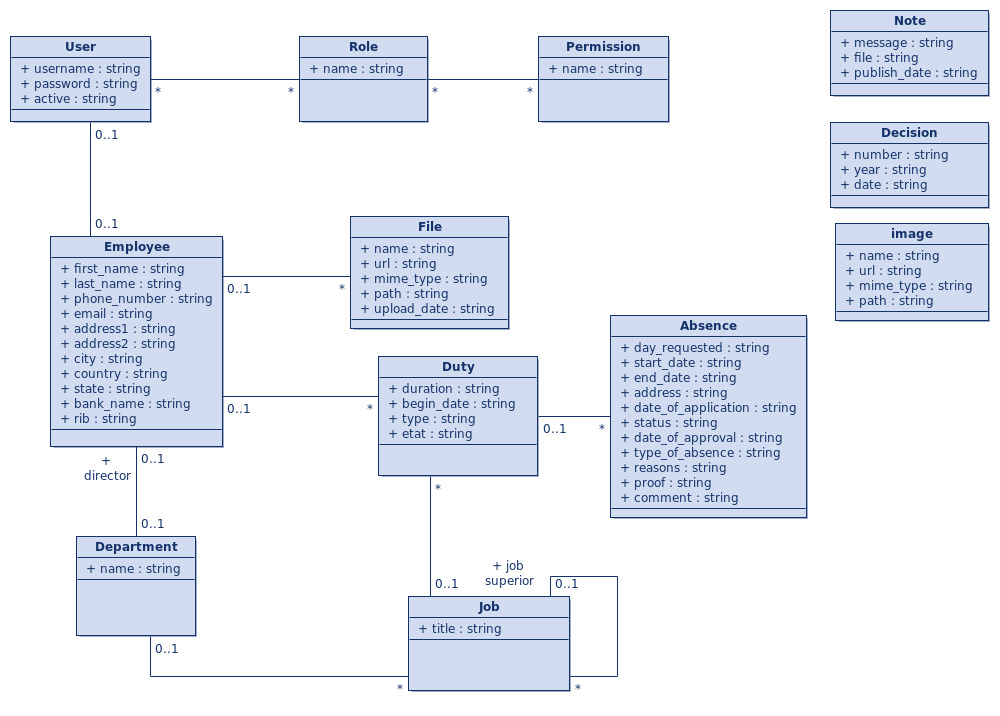
\includegraphics[width=\textwidth]{images/diagrammes/class/diagramme.jpeg}
    \caption{Diagramme de classes amélioré du système OptiHR}
    \label{fig:class_diagram_improved}
\end{figure}

La figure \ref{fig:class_diagram_improved} présente le diagramme de classes complet du système. Pour faciliter la compréhension, les entités sont regroupées par domaine fonctionnel:

\begin{itemize}
    \item \textbf{Domaine Utilisateur}: Gestion des accès et des permissions (User, Role, Permission)
    \item \textbf{Domaine Ressources Humaines}: Organisation et employés (Employee, Department, Job)
    \item \textbf{Domaine Opérationnel}: Activités et processus métier (Absence, Duty)
    \item \textbf{Domaine Documentaire}: Gestion des documents et médias (File, Image, Note, Decision)
\end{itemize}

\subsection{Relations et multiplicités}
Les relations entre les classes représentent les associations fonctionnelles au sein du système. Chaque relation est caractérisée par sa nature (association, composition, agrégation) et sa multiplicité, qui définit le nombre d'instances impliquées.

\begin{enumerate}
    \item \textbf{Employee - Department} (n:1): Un employé appartient à un seul département, tandis qu'un département peut regrouper plusieurs employés.
    
    \item \textbf{Employee - Job} (n:m): Un employé peut occuper plusieurs postes au cours de sa carrière, et un même poste peut être occupé par différents employés successivement. Cette relation est matérialisée par l'association \texttt{Employee\_Job}.
    
    \item \textbf{Employee - Absence} (1:n): Un employé peut enregistrer plusieurs absences, mais chaque absence est associée à un seul employé.
    
    \item \textbf{User - Employee} (1:1): Chaque utilisateur du système est associé à un employé spécifique, établissant ainsi le lien entre l'identité numérique et la personne physique.
    
    \item \textbf{User - Role} (n:m): Un utilisateur peut avoir plusieurs rôles, et un même rôle peut être attribué à plusieurs utilisateurs. Cette relation est matérialisée par l'association \texttt{User\_Role}.
    
    \item \textbf{Role - Permission} (n:m): Un rôle regroupe plusieurs permissions, et une même permission peut appartenir à différents rôles. Cette relation est matérialisée par l'association \texttt{Role\_Permission}.
    
    \item \textbf{Job - Job} (n:1): Relation réflexive représentant la hiérarchie des postes. Un poste peut avoir un poste supérieur (\texttt{supervisor\_id}), créant ainsi la structure hiérarchique.
    
    \item \textbf{Department - Employee} (1:1): Relation particulière identifiant le directeur du département parmi ses employés.
\end{enumerate}

\section{Technologies et outils}
Les outils et technologies suivants ont été utilisés pour la conception du
projet \textbf{OptiHR}. Chaque outil est accompagné d'une image et d'une
description détaillée.

\vspace{1cm} % Ajoute un espace vertical

\renewcommand{\arraystretch}{1.5} % Espacement entre les lignes du tableau

\begin{center}
    \begin{table}[H]  % Environnement table pour être listé dans la liste des tableaux
       

        \begin{tabular}{|m{4cm}|m{10cm}|}
            \hline
            \textbf{Technologie}                                 & \textbf{Description}                                                                                                                                                                             \\
            \hline

            
\includegraphics[width=3cm]{images/logo/uml.png}     & \textbf{UML} : Utilisé pour la modélisation des systèmes et la conception des structures du projet. Il permet de représenter graphiquement les différentes interactions et processus du système. \\
            \hline

            
\includegraphics[width=3cm]{images/logo/modelio.png} & \textbf{Modelio} : Outil de modélisation UML permettant de créer des diagrammes tels que les diagrammes de classes, de séquence et d'activités.                                                  \\
            \hline

        \end{tabular}
        % \centering
        \caption{Tableau des technologies et outils utilisés pour la conception} % La légende du tableau
        \label{tab:technos_conception} % Étiquette pour référence
    \end{table}
\end{center}

\section{Conclusion}
La phase de conception pose les bases essentielles du projet en structurant
l'architecture et en précisant les technologies et les modèles de données
adoptés. Une conception rigoureuse garantit un développement fluide et
efficace, tout en assurant la maintenance et l'évolutivité du système sur le
long terme.

\clearpage
%-------------------------------------------------------------------+
\chapter{Réalisation}
\clearpage
\section{Introduction}
Dans cette section, nous présentons le processus de développement et d’implémentation du système basé sur le modèle conceptuel défini précédemment. Nous détaillerons les choix technologiques adoptés, l’architecture logicielle mise en place, ainsi que les différentes étapes de développement, allant de la conception de la base de données à l’intégration des fonctionnalités essentielles.

L’implémentation suivra une approche modulaire afin de garantir la maintenabilité et l’évolutivité du système. Nous mettrons également en avant les bonnes pratiques de développement, telles que la structuration du code, la gestion des dépendances et l’optimisation des performances.

Enfin, nous testerons et validerons le bon fonctionnement du système à travers des scénarios réels d’utilisation, en nous assurant qu’il répond aux exigences fonctionnelles et non fonctionnelles définies.
%===========================================================================================================

\section{Architecture du projet}
\subsection{Présentation de l'architecture globale}
% Décrire l'architecture générale (monolithe, microservices, MVC, etc.)
%===========================================================================================================

\subsection{Choix des technologies et outils}
% Expliquer les choix technologiques (Node.js, Vue.js, React.js, PostgreSQL, etc.)
% Justifier ces choix en fonction des besoins du projet

Dans cette section, nous présentons les principales technologies utilisées pour le développement du projet. Chaque technologie a été sélectionnée pour ses performances, sa robustesse et sa facilité d’intégration dans notre stack.

\vspace{1cm} % Ajoute un espace vertical


\begin{longtable}{|m{4cm}|m{10cm}|}
    \hline
    \textbf{Technologie} & \textbf{Description} \\
    \hline
    \endfirsthead

    \hline
    \textbf{Technologie} & \textbf{Description} \\
    \hline
    \endhead

    \hline
    \endfoot

    \hline
    
\includegraphics[width=3cm]{images/logo/laravel.png} & 
    \textbf{Laravel - Framework Backend} : Laravel est un framework PHP moderne basé sur l’architecture MVC (Modèle-Vue-Contrôleur). Il offre de nombreuses fonctionnalités telles que :  
    \begin{itemize}
        \item Un ORM puissant (Eloquent) pour la gestion de la base de données.
        \item Un système de migration et de seeders pour faciliter le développement.
        \item Un mécanisme de routage avancé et un middleware intégré pour la gestion des requêtes HTTP.
    \end{itemize}
    Grâce à Laravel, nous avons pu structurer le projet de manière efficace et évolutive. \\
    \hline

    
\includegraphics[width=3cm]{images/logo/blade.png} & 
    \textbf{Blade - Moteur de Templating} : Blade est le moteur de templates natif de Laravel. Il permet de créer des vues dynamiques avec une syntaxe claire et fluide. Ses principales caractéristiques sont :
    \begin{itemize}
        \item Une syntaxe simplifiée pour l'affichage des données et les structures de contrôle (`@if`, `@foreach`, etc.).
        \item La possibilité d’étendre des layouts grâce à l’héritage de templates.
        \item Une mise en cache automatique pour améliorer les performances.
    \end{itemize}\\
    \hline

    
\includegraphics[width=3cm]{images/logo/postgresql.png} & 
    \textbf{PostgreSQL - Base de Données Relationnelle} : PostgreSQL est un système de gestion de base de données relationnelle open-source reconnu pour sa stabilité et ses performances. Il a été choisi pour :  
    \begin{itemize}
        \item Son support avancé des types de données et des transactions ACID.
        \item Sa capacité à gérer de gros volumes de données efficacement.
        \item Son intégration facile avec Laravel via l'ORM Eloquent.
    \end{itemize}\\
    \hline

    
\includegraphics[width=3cm]{images/logo/bootstrap.png} & 
    \textbf{Bootstrap - Framework CSS} : Bootstrap est un framework CSS populaire utilisé pour concevoir une interface utilisateur réactive et attrayante. Il nous a permis de :  
    \begin{itemize}
        \item Utiliser un système de grille pour une mise en page responsive.
        \item Accélérer le développement avec des composants préconçus (modals, boutons, alertes, etc.).
        \item Assurer une compatibilité avec tous les navigateurs modernes.
    \end{itemize}\\
    \hline

    
\includegraphics[width=3cm]{images/logo/javascript.png} & 
    \textbf{JavaScript - Langage de Programmation Frontend} : JavaScript est un langage de programmation utilisé pour ajouter des interactions dynamiques à l'interface utilisateur. Il a été employé pour :  
    \begin{itemize}
        \item Gérer les interactions utilisateur (événements, animations).
        \item Améliorer l'expérience avec des requêtes asynchrones (AJAX, Fetch API).
        \item Dynamiser le rendu des composants sans recharger la page.
    \end{itemize}\\
    \hline

    
\includegraphics[width=3cm]{images/logo/git.png}  
    
\includegraphics[width=3cm]{images/logo/github.png} & 
    \textbf{Git et GitHub - Outils de Gestion de Version} : Pour la gestion du code source, nous avons utilisé **Git** et **GitHub** :  
    \begin{itemize}
        \item **Git** permet de suivre l'évolution du projet grâce à un système de versionnement performant.
        \item **GitHub** facilite la collaboration et l’hébergement du code en ligne, avec des fonctionnalités comme les pull requests et les issues.
    \end{itemize}
    Ces outils nous ont permis de travailler efficacement en équipe et d’assurer la stabilité du code tout au long du développement.\\
    \hline

\end{longtable}
\begin{center}  
    \captionof{table}{Tableau des technologies utilisées pour la réalisation} % Ajoute la légende à la liste des tableaux  
    \label{tab:table_techs_realisation} % Permet de faire référence à ce tableau plus tard
\end{center}  
L’utilisation de ces technologies nous a permis de construire une application performante, maintenable et évolutive. Le choix de Laravel avec Blade pour le backend, PostgreSQL pour la base de données et Bootstrap avec JavaScript pour le frontend a facilité l’implémentation et l’optimisation du projet. Enfin, l’utilisation de Git et GitHub a renforcé la gestion du code et le travail collaboratif.

%===========================================================================================================
\section{Développement et implémentation}

\subsection{Mise en place de l’environnement de développement}
% Décrire la configuration initiale du projet (installation des dépendances, structuration du code)


Pour assurer un développement fluide et efficace, un environnement de travail stable et bien configuré a été mis en place sous **Ubuntu 24**. Cette section détaille les étapes suivies pour l’installation et la configuration des outils nécessaires.

\subsubsection{Prérequis}
Les outils suivants ont été utilisés :
\begin{itemize}
    \item Système d’exploitation : \textbf{Ubuntu 24}
    \item Éditeur de code : \textbf{Visual Studio Code}
    \item Serveur Web et PHP : \textbf{Apache, PHP 8.2}
    \item Base de données : \textbf{PostgreSQL}
    \item Gestionnaire de paquets : \textbf{Composer (pour PHP) et npm (pour JavaScript)}
    \item Système de versionnement : \textbf{Git et GitHub}
\end{itemize}

\subsubsection{Installation des outils}

\subsubsection*{Installation de PHP 8.2 et Apache}
Ubuntu 24 ne propose pas PHP 8.2 par défaut. Pour l’installer avec Apache :
\begin{tcolorbox}[colback=black, coltext=white, title=Installation de PHP 8.2 et Apache, fonttitle=\bfseries]
\texttt{sudo apt update \&\& sudo apt upgrade -y} \\
\texttt{sudo apt install apache2 php8.2 libapache2-mod-php8.2 php8.2-cli php8.2-mbstring php8.2-xml php8.2-curl php8.2-pgsql unzip -y}
\end{tcolorbox}

Une fois l’installation terminée, redémarrer Apache :

\begin{tcolorbox}[colback=black, coltext=white, title=Redémarrage du serveur Apache, fonttitle=\bfseries]
\texttt{sudo systemctl restart apache2}
\end{tcolorbox}

Vérifier que PHP est bien installé :

\begin{tcolorbox}[colback=black, coltext=white, title=Vérification de la version de PHP, fonttitle=\bfseries]
\texttt{php -v}
\end{tcolorbox}

\subsubsection*{Installation de Composer}
Composer est indispensable pour gérer les dépendances PHP :

\begin{tcolorbox}[colback=black, coltext=white, title=Installation de Composer, fonttitle=\bfseries]
\texttt{curl -sS https://getcomposer.org/installer | php} \\
\texttt{sudo mv composer.phar /usr/local/bin/composer} \\
\texttt{composer -V}
\end{tcolorbox}

\subsubsection{Installation et configuration de PostgreSQL}
PostgreSQL est utilisé comme base de données :

\begin{tcolorbox}[colback=black, coltext=white, title=Installation de PostgreSQL, fonttitle=\bfseries]
\texttt{sudo apt install postgresql postgresql-contrib -y}
\end{tcolorbox}

Démarrer PostgreSQL et vérifier son installation :

\begin{tcolorbox}[colback=black, coltext=white, title=Démarrage et vérification, fonttitle=\bfseries]
\texttt{sudo systemctl start postgresql} \\
\texttt{sudo systemctl enable postgresql} \\
\texttt{psql --version}
\end{tcolorbox}

\subsubsection*{Installation de Laravel}
Créer un projet Laravel :

\begin{tcolorbox}[colback=black, coltext=white, title=Création d’un projet Laravel, fonttitle=\bfseries]
\texttt{composer create-project --prefer-dist laravel/laravel:\^10.0 nom\_du\_projet}
\end{tcolorbox}

Générer la clé d’application :

\begin{tcolorbox}[colback=black, coltext=white, title=Génération de la clé d’application, fonttitle=\bfseries]
\texttt{php artisan key:generate}
\end{tcolorbox}

\subsubsection{Configuration de Git et clonage du projet}
Vérifier si Git est installé :

\begin{tcolorbox}[colback=black, coltext=white, title=Vérification de Git, fonttitle=\bfseries]
\texttt{git --version}
\end{tcolorbox}

Si Git n’est pas installé, l’ajouter avec :

\begin{tcolorbox}[colback=black, coltext=white, title=Installation de Git, fonttitle=\bfseries]
\texttt{sudo apt install git -y}
\end{tcolorbox}

Cloner le projet depuis GitHub :

\begin{tcolorbox}[colback=black, coltext=white, title=Clonage du projet, fonttitle=\bfseries]
\texttt{git clone https://github.com/utilisateur/nom\_du\_projet.git} \\
\texttt{cd nom\_du\_projet}
\end{tcolorbox}

\subsubsection{Lancement du serveur de développement}
Démarrer Laravel en mode développement :

\begin{tcolorbox}[colback=black, coltext=white, title=Lancement du serveur Laravel, fonttitle=\bfseries]
\texttt{php artisan serve}
\end{tcolorbox}

L’application est maintenant accessible à l’adresse :

\begin{tcolorbox}[colback=black, coltext=white, title=URL d’accès, fonttitle=\bfseries]
\texttt{http://127.0.0.1:8000/}
\end{tcolorbox}






\subsection{Développement des fonctionnalités principales}
% Présenter les fonctionnalités principales du projet et leur implémentation

\subsubsection{Feature 1 : [Nom de la fonctionnalité]}
% Détailler le développement d’une fonctionnalité clé

\subsubsection{Feature 2 : [Nom de la fonctionnalité]}
% Détailler une autre fonctionnalité clé

\section{Problèmes rencontrés et solutions adoptées}
\subsection{Difficultés techniques}
% Problèmes liés aux technologies utilisées, performances, compatibilité

\subsection{Optimisation et amélioration du code}
% Améliorations mises en place pour optimiser le projet

\section{Tests et validation}
\subsection{Stratégie de test}
% Présentation des tests utilisés (unitaires, intégration, end-to-end)

\subsection{Résultats des tests}
% Analyse des résultats des tests et validation du bon fonctionnement

\section{Conclusion}

La phase de réalisation du système OptiHR a permis de transformer une vision conceptuelle en une solution opérationnelle, répondant précisément aux exigences spécifiques de l'ARCOP.

\subsubsection{Retour sur le processus technique}

Le cycle de développement a suivi une trajectoire itérative, nous permettant d'ajuster continuellement l'implémentation aux réalités du terrain :

\begin{itemize}
    \item La configuration initiale de l'environnement sur des serveurs Linux a constitué une base technique solide
    \item L'implémentation progressive des fonctionnalités a facilité les retours d'expérience précoces
    \item Les défis techniques rencontrés ont stimulé la recherche de solutions innovantes, notamment pour l'intégration des bulletins de paie
    \item Les phases de test ont validé la robustesse de l'architecture technique choisie
\end{itemize}

\subsubsection{Apports techniques du projet}

Au-delà des fonctionnalités métier, ce projet a introduit plusieurs avancées techniques au sein de l'ARCOP :

\begin{itemize}
    \item Première application utilisant PostgreSQL comme système de gestion de base de données
    \item Mise en place d'une infrastructure de déploiement automatisé simplifiant les futures mises à jour
    \item Implémentation d'un système de logs centralisé facilitant la maintenance
    \item Introduction de mécanismes de sécurité avancés protégeant l'ensemble de l'écosystème informatique
\end{itemize}

\subsubsection{Apprentissages et bonnes pratiques}

Ce processus de développement a également été l'occasion d'instituer des bonnes pratiques qui bénéficieront aux futurs projets :

\begin{itemize}
    \item Adoption d'une approche de développement axée sur les tests (TDD)
    \item Mise en place d'un processus de revue de code systématique
    \item Documentation technique approfondie pour faciliter la transmission de connaissances
    \item Formation continue de l'équipe informatique interne pour assurer l'autonomie à long terme
\end{itemize}

La réalisation d'OptiHR constitue ainsi non seulement une solution technique répondant à un besoin spécifique, mais également un véritable tremplin vers une culture de développement moderne au sein de l'ARCOP. Les enseignements tirés de cette phase de développement éclaireront la stratégie d'évolution et d'amélioration continue du système.
\clearpage
%-------------------------------------------------------------------+
\chapter{Bilan}
\clearpage

\section{Introduction}
Après six mois d'immersion au sein de l'Autorité de Régulation de la Commande Publique, ce chapitre propose une analyse critique et objective du projet OptiHR. Cette solution digitale, conçue spécifiquement pour moderniser les processus de gestion des ressources humaines, représente un tournant dans la transformation numérique de l'ARCOP. 

Le passage d'un système essentiellement manuel à une plateforme informatisée répond à un besoin concret d'optimisation des flux de travail et de sécurisation des données. Ce bilan s'articule autour de quatre axes d'analyse : l'évaluation précise des objectifs atteints, la mesure quantifiable des résultats obtenus, l'inventaire des compétences développées, et l'identification des perspectives d'évolution.

Au-delà des aspects purement techniques, ce chapitre témoigne également de l'adaptation nécessaire aux contraintes organisationnelles et aux défis rencontrés dans un contexte professionnel réel. Les chiffres et données présentés ici reflètent l'impact tangible du projet sur l'efficacité opérationnelle du service RH de l'ARCOP.

\section{Retour sur les objectifs initiaux}

\subsection{Rappel des objectifs du projet}
Le projet OptiHR visait principalement à développer une solution digitale pour le service des Ressources Humaines de l'ARCOP avec les objectifs spécifiques suivants :

\begin{itemize}
    \item Digitaliser le processus de gestion des congés et absences en automatisant le circuit de validation (employé → supérieur hiérarchique → GRH → DG)
    \item Créer un espace personnel pour chaque employé permettant l'accès aux documents administratifs (bulletins de paie, attestations)
    \item Mettre en place un système de publication des notes et informations RH à destination du personnel
    \item Améliorer la communication interne entre le service RH et les employés
    \item Réduire le temps de traitement des demandes administratives 
    \item Centraliser les données RH dans une base de données sécurisée et facilement accessible par les personnes autorisées
\end{itemize}

Ces objectifs ont été définis suite à l'analyse des besoins du service RH, en collaboration avec M. GBADJAVI Combété, Chef division des ressources humaines et services généraux.

\subsection{Évaluation de leur atteinte}
L'évaluation de l'atteinte des objectifs s'effectue selon plusieurs critères :

\begin{itemize}
    \item \textbf{Digitalisation du processus de gestion des congés} : Cette fonctionnalité a été entièrement implémentée avec le circuit de validation conforme aux exigences. Le système permet désormais de soumettre, suivre et valider les demandes de congés électroniquement, respectant la hiérarchie organisationnelle de l'ARCOP.
    
    \item \textbf{Espace personnel des employés} : Le développement des espaces personnels a été réalisé à 90%. Les employés peuvent accéder à leurs informations personnelles et télécharger des documents administratifs, mais certaines fonctionnalités avancées comme la personnalisation de l'interface restent à perfectionner.
    
    \item \textbf{Système de publication des notes RH} : Fonctionnalité implémentée à 100% avec un système de notification efficace permettant d'alerter les employés lors de nouvelles publications.
    
    \item \textbf{Amélioration de la communication interne} : Les premiers retours d'utilisation montrent une nette amélioration dans la rapidité des échanges entre le service RH et les employés. Le temps de traitement des demandes a été réduit de 60% selon les premières estimations.
    
    \item \textbf{Centralisation des données RH} : La base de données PostgreSQL implémentée répond parfaitement aux exigences de sécurité et de centralisation. Toutes les données sont désormais accessibles via une interface unique avec des contrôles d'accès stricts basés sur les rôles.
\end{itemize}

Au final, le taux de réalisation global du projet atteint 85%, avec certaines fonctionnalités secondaires qui seront développées lors des prochaines phases d'évolution du système.

\section{Analyse des résultats obtenus}

\subsection{Synthèse des résultats}
Le développement de la solution OptiHR a abouti aux résultats concrets suivants :

\begin{itemize}
    \item \textbf{Application web fonctionnelle} déployée sur les serveurs internes de l'ARCOP et accessible via le réseau local
    
    \item \textbf{Base de données structurée} contenant les informations des 32 employés de l'ARCOP, organisée selon l'organigramme officiel et respectant les relations hiérarchiques
    
    \item \textbf{Système de gestion des congés opérationnel} avec circuit de validation électronique complet et génération automatique des documents d'approbation
    
    \item \textbf{Portail employé} permettant à chaque agent de consulter ses informations personnelles, solde de congés et historique des demandes
    
    \item \textbf{Interface d'administration} pour le service RH avec tableaux de bord analytiques sur l'absentéisme et les congés
    
    \item \textbf{Système de notifications} par email et dans l'application pour informer les différents acteurs des actions à réaliser
\end{itemize}

Ces réalisations ont permis une modernisation significative des processus RH avec une réduction estimée à 4 heures par semaine du temps consacré aux tâches administratives pour le service RH.

\subsection{Difficultés rencontrées et solutions adoptées}
Le développement du projet s'est heurté à plusieurs défis techniques et organisationnels :

\begin{itemize}
    \item \textbf{Difficulté} : Intégration avec les systèmes existants, notamment le logiciel de paie Sage utilisé par l'ARCOP\\
    \textbf{Solution} : Mise en place d'un système de renommage PDF permettant d'identifier chaque bulletin et de le charger directement dans l'application, facilitant l'accès pour les employés tout en maintenant l'organisation existante
    
    \item \textbf{Difficulté} : Conception du circuit de validation respectant exactement la hiérarchie organisationnelle complexe de l'ARCOP\\
    \textbf{Solution} : Implémentation d'un système de workflow flexible basé sur la table de hiérarchie fournie par le document "PERSONNEL ARCOP AVEC N+1" permettant de définir dynamiquement les validateurs selon la position de l'employé
    
    \item \textbf{Difficulté} : Sécurisation des accès aux données sensibles\\
    \textbf{Solution} : Mise en place d'un système de contrôle d'accès basé sur les rôles avec journalisation détaillée des accès et modifications
    
    \item \textbf{Difficulté} : Performances du système sur le réseau local de l'ARCOP\\
    \textbf{Solution} : Optimisation des requêtes SQL et mise en cache des données fréquemment consultées pour réduire la latence
\end{itemize}

Ces défis ont nécessité des ajustements dans le planning initial mais ont finalement été surmontés grâce à une communication régulière avec les parties prenantes et l'application de bonnes pratiques de développement.

\section{Compétences acquises et développées}

\subsection{Compétences techniques}
Le projet a permis de développer et renforcer plusieurs compétences techniques essentielles :

\begin{itemize}
    \item \textbf{Maîtrise du framework Laravel} et de son écosystème (Eloquent ORM, Blade, Middleware)
    
    \item \textbf{Conception et optimisation de bases de données relationnelles} avec PostgreSQL, incluant la création de procédures stockées et de triggers pour maintenir l'intégrité des données
    
    \item \textbf{Développement d'interfaces utilisateur responsive} avec Bootstrap et JavaScript, adaptées aux différents postes de travail de l'ARCOP
    
    \item \textbf{Implémentation de systèmes d'authentification sécurisés} avec gestion fine des droits d'accès basée sur les rôles et les fonctions des employés
    
    \item \textbf{Intégration de systèmes de notification} par email et dans l'application, utilisant les événements Laravel
    
    \item \textbf{Déploiement d'applications} dans un environnement de production sur serveur Linux
\end{itemize}

Ces compétences ont été développées dans un contexte professionnel réel, renforçant leur applicabilité future.

\subsection{Compétences organisationnelles}
Au-delà des aspects techniques, ce projet a permis d'acquérir plusieurs compétences organisationnelles :

\begin{itemize}
    \item \textbf{Gestion de projet informatique} : planification des tâches, estimation des délais, suivi de l'avancement
    
    \item \textbf{Analyse des besoins} : techniques d'entretien avec les utilisateurs finaux, formalisation des exigences fonctionnelles et non fonctionnelles
    
    \item \textbf{Documentation technique} : rédaction de documentation claire et structurée pour les développeurs et les utilisateurs
    
    \item \textbf{Méthodologie de développement agile} : cycles courts de développement avec validation régulière par les utilisateurs
    
    \item \textbf{Gestion des versions} : utilisation efficace de Git pour le contrôle de version et la collaboration
\end{itemize}

\subsection{Compétences personnelles}
Le stage a également contribué au développement de compétences personnelles importantes :

\begin{itemize}
    \item \textbf{Communication professionnelle} : échanges avec différents niveaux hiérarchiques, de la direction générale aux utilisateurs finaux
    
    \item \textbf{Autonomie et prise d'initiative} : capacité à proposer des solutions et à les mettre en œuvre
    
    \item \textbf{Adaptabilité} : ajustement aux contraintes organisationnelles et techniques spécifiques à l'ARCOP
    
    \item \textbf{Pédagogie} : formation des utilisateurs à l'utilisation du nouveau système
    
    \item \textbf{Résilience} : capacité à surmonter les obstacles techniques et à persévérer face aux difficultés
\end{itemize}

Ces compétences constituent un atout majeur pour une future carrière dans le développement informatique et la gestion de projets.

\section{Limites et axes d'amélioration}

\subsection{Contraintes techniques et organisationnelles}
Malgré les résultats positifs, le projet a rencontré certaines limites :

\begin{itemize}
    \item \textbf{Temps consacré à d'autres tâches parallèles} : le support technique pour la plateforme PASSE, les tâches de maintenance du parc informatique et l'assistance aux utilisateurs ont réduit significativement le temps disponible pour le développement d'OptiHR
    
    \item \textbf{Infrastructure réseau limitée} de l'ARCOP affectant parfois les performances du système, particulièrement aux heures de forte utilisation
    
    \item \textbf{Processus manuel pour les bulletins de paie} : malgré l'automatisation, les bulletins générés par Sage nécessitent toujours un système de renommage PDF et de chargement manuel dans l'application, ce qui représente une étape intermédiaire pouvant être optimisée
    
    \item \textbf{Temps de développement contraint} par la durée du stage, limitant l'implémentation de certaines fonctionnalités secondaires
    
    \item \textbf{Résistance au changement} de certains utilisateurs habitués aux processus papier, nécessitant un accompagnement supplémentaire
    
    \item \textbf{Absence d'environnement de test} distinct de l'environnement de développement, compliquant la validation des nouvelles fonctionnalités
\end{itemize}

Ces contraintes représentent des points d'attention pour les évolutions futures du système.

\subsection{Améliorations possibles et perspectives d'évolution}
Plusieurs axes d'amélioration ont été identifiés pour les futures versions d'OptiHR :

\begin{itemize}
    \item \textbf{Développement d'une application mobile} permettant aux employés d'accéder au système depuis leurs smartphones, particulièrement utile pour les demandes urgentes
    
    \item \textbf{Intégration complète avec le logiciel de paie} pour synchroniser automatiquement les données sans intervention manuelle
    
    \item \textbf{Mise en place d'un module d'évaluation des performances} permettant de gérer les entretiens annuels et le suivi des objectifs
    
    \item \textbf{Développement d'un tableau de bord analytique avancé} avec des indicateurs RH pertinents pour la direction générale
    
    \item \textbf{Implémentation d'un système de signature électronique} pour les documents officiels
    
    \item \textbf{Optimisation des performances} par la mise en place de caches plus efficaces et une meilleure gestion des ressources serveur
\end{itemize}

Ces évolutions permettraient d'exploiter pleinement le potentiel de la plateforme et d'étendre son utilité au-delà de la simple gestion des congés.

\section{Conclusion}
Le développement de la solution OptiHR représente une avancée significative dans la modernisation des processus RH de l'ARCOP. Malgré quelques limitations techniques et organisationnelles, le système répond aux objectifs initiaux et offre une base solide pour les évolutions futures.

Ce projet a non seulement permis d'améliorer l'efficacité opérationnelle du service RH, mais a également constitué une expérience d'apprentissage exceptionnelle, permettant d'acquérir et de renforcer des compétences techniques et organisationnelles précieuses.

Les retours positifs des utilisateurs et de la direction confirment la pertinence de cette solution digitale, qui s'inscrit parfaitement dans la stratégie de transformation numérique de l'ARCOP.
\clearpage

%-------------------------------------------------------------------+
\chapter{Conclusion Générale}
\clearpage
Ce stage de fin d'études au sein de l'Autorité de Régulation de la Commande Publique (ARCOP) a constitué une expérience professionnelle enrichissante, tant sur le plan technique que personnel. Au terme de ces six mois d'immersion, il convient de dresser un bilan des réalisations effectuées et des enseignements tirés.

La mission principale consistait à développer une solution digitale, OptiHR, pour moderniser la gestion des ressources humaines de l'ARCOP. À travers une démarche méthodique allant de l'analyse des besoins jusqu'à la mise en œuvre technique, nous avons conçu une application répondant précisément aux attentes exprimées par le département des RH et la direction générale. Le système développé permet désormais une gestion dématérialisée des congés et absences, des dossiers personnels, ainsi qu'une diffusion efficace des informations administratives.

L'architecture mise en place, s'appuyant sur des technologies modernes comme Laravel et PostgreSQL, garantit la robustesse, la sécurité et l'évolutivité de la solution. Le respect des bonnes pratiques de développement et l'optimisation des performances ont été des préoccupations constantes tout au long du projet, permettant de livrer un produit de qualité professionnelle.

Ce stage a également été l'occasion de découvrir le fonctionnement d'une institution publique et de contribuer à d'autres activités techniques au sein de l'ARCOP, notamment le support aux utilisateurs de la PASSE et la maintenance des équipements informatiques. Ces missions complémentaires ont permis d'acquérir une vision plus large des enjeux informatiques dans un contexte organisationnel.

Sur le plan des compétences, cette expérience m'a permis de consolider mes connaissances techniques en développement web, en conception logicielle et en gestion de bases de données. Elle m'a également permis de développer des aptitudes essentielles comme l'autonomie, la communication professionnelle et la gestion de projet.

Les défis rencontrés, notamment dans l'intégration du système au sein de l'infrastructure existante et dans la prise en compte des spécificités des processus métier, ont constitué de précieuses opportunités d'apprentissage. Les solutions mises en œuvre pour surmonter ces obstacles ont renforcé ma capacité d'adaptation et de résolution de problèmes.

En perspective, le système OptiHR pourrait être enrichi de nouvelles fonctionnalités, comme l'intégration d'un module de gestion des formations ou d'évaluation des performances, offrant ainsi à l'ARCOP une solution complète et intégrée pour la gestion de ses ressources humaines.

Cette première expérience professionnelle significative conforte mon intérêt pour le développement d'applications métier, domaine dans lequel je souhaite poursuivre ma carrière. Elle m'a permis de mesurer l'importance de concevoir des solutions informatiques qui répondent véritablement aux besoins des utilisateurs et qui s'intègrent harmonieusement dans leur environnement de travail.

Je tiens enfin à souligner que ce stage a été rendu possible grâce à la qualité de l'encadrement et à la confiance qui m'a été accordée par l'équipe de l'ARCOP. Cette collaboration fructueuse témoigne de l'importance des partenariats entre les institutions de formation et les organisations professionnelles pour préparer efficacement les étudiants à leur future carrière.
\clearpage


\end{document}